\documentclass[a4paper,10pt]{article}

\usepackage[utf8]{inputenc}
\usepackage[T1]{fontenc} 
\usepackage{amsfonts,amssymb,amsthm}
\usepackage{amsmath,amscd}
\usepackage{algorithmicx,algorithm}
\usepackage[noend]{algpseudocode}
\usepackage{fullpage}
\usepackage{subcaption}
\usepackage{bm}
\usepackage{bbm}
\usepackage{centernot} 
\usepackage{enumerate} 
\usepackage{parskip}
\usepackage{pb-diagram} 
\usepackage{mathrsfs}
\usepackage[OT2,T1]{fontenc}
\usepackage{seqsplit}
\usepackage{enumitem}
\usepackage{color}
\usepackage{array}
\usepackage{verbatim}
\usepackage{url}
\usepackage{tikz, graphicx}
\usepackage{mathtools} %For mapsto
\usetikzlibrary{shapes, arrows, calc, positioning}
\usepackage{wrapfig, blindtext}
\usepackage{mleftright}
\usepackage{pgffor} %The for loop
%\usepackage{euler} %For the \mathscr
\usepackage{float} % For figure
\usepackage{hyperref}
%Bibtex
% \usepackage{cite}
% \usepackage[nottoc]{tocbibind}
\usepackage{natbib}
\bibliographystyle{abbrvnat}
% \bibpunct{(}{)}{;}{a}{,}{,}


%encadre
\usepackage{tcolorbox}
\usepackage{cleveref}
\newcommand{\todo}[1]{\textcolor{red}{\textbf{TODO:} #1}}

\DeclareMathOperator*{\argmin}{argmin}
\DeclareMathOperator*{\argmax}{argmax}


\newtheorem{theorem}{Theorem}[section]
\newtheorem{corollary}{Corollary}[theorem]
\newtheorem{lemma}[theorem]{Lemma}
\newtheorem{proposition}[theorem]{Proposition}
\newtheorem{assumption}[theorem]{Assumption}
\newtheorem{remark}{Remark}

\theoremstyle{definition}
\newtheorem{definition}{Definition}[section]
\newtheorem{example}{Example}[section]

\newtcolorbox{mybox}[1][]{colback=green!5!white, colframe=black, coltitle=white, fonttitle=\bfseries}
\allowdisplaybreaks
\newcommand{\eqdef}{\overset{\text{\scriptsize{def}}}{=}}

% Real
\newcommand{\R}{\mathbb{R}}
\newcommand{\Z}{\mathbb{Z}}
\newcommand{\N}{\mathbb{N}}

% Expectation, probability, Gaussian, Covariance and Variance
\newcommand{\E}[1]{\mathbb{E} \left[ {#1} \right] }
\newcommand{\EE}[2]{\mathbb{E}_{#2} \left[ {#1} \right] }
\newcommand{\Ec}[2]{\mathbb{E}_{{#2}} \left[ {#1} \right] }

\newcommand{\Pro}[1]{\mathbb{P}\left( {#1} \right) }
\newcommand{\Normal}[1]{\mathcal{N}\left( {#1} \right)}
\newcommand{\Cov}[1]{\mathrm{Cov}\left( {#1} \right)}
\newcommand{\Var}[1]{\mathrm{Var}\left( {#1} \right)}

% Linear algebra
\renewcommand{\ker}[1]{\mathrm{ker}\left( {#1} \right)}
\newcommand{\rank}[1]{\mathrm{rank}\left( {#1} \right)}
\newcommand{\supp}[1]{\mathrm{supp}\left( {#1} \right)}
\newcommand{\Id}{\mathrm{I}}
\newcommand{\trace}[1]{\mathrm{tr}\left( #1 \right)}
\newcommand{\diag}[1]{\mathrm{diag}\left( #1 \right)}
\newcommand{\diam}[1]{\mathrm{diam}\left( #1 \right)}
\newcommand{\norm}[1]{\left\| #1 \right \|}
\newcommand{\inner}[1]{\left\langle #1 \right\rangle}

% bold symbol
\newcommand{\bs}[1]{\boldsymbol{#1}}

% Manifold
\newcommand{\M}{\mathcal{M}}
\newcommand{\x}{\boldsymbol{x}}
\newcommand{\z}{\boldsymbol{z}}
\renewcommand{\i}{\boldsymbol{i}}
\newcommand{\w}{\boldsymbol{w}}
\newcommand{\beps}{\boldsymbol{\epsilon}}
\newcommand{\eps}{\epsilon}
\newcommand{\A}{\boldsymbol{A}}
\newcommand{\y}{\boldsymbol{y}}
\newcommand{\n}{\boldsymbol{n}}
\newcommand{\0}{\boldsymbol{0}}
\renewcommand{\Im}[1]{\mathrm{Im} \left( {#1}  \right)}


\newcommand{\X}{\mathcal{X}}
\newcommand{\Y}{\mathcal{Y}}
\renewcommand{\H}{\mathcal{H}}
\newcommand{\D}{\mathcal{D}}
\renewcommand{\det}[1]{\mathrm{det}\left( #1 \right)}
\newcommand{\Tx}{T^{\X}}
\newcommand{\Ty}{T^{\Y}}




% \usepackage{natbib}
% \usepackage{geometry}
% \usepackage{graphicx} % Required for inserting images
% \usepackage{amsmath}
% \usepackage{amssymb}
% \usepackage{amsthm}
% \usepackage{mathtools}
% \usepackage{enumitem}
% \usepackage{bbm}
% \usepackage{xcolor}
% \usepackage{hyperref}
% \usepackage{cleveref} % Pour pouvoir utiliser cref


% \bibliographystyle{abbrvnat}

% \theoremstyle{definition} % Style pour les définitions
% \newtheorem{definition}{Definition}[section]

% \theoremstyle{definition} % Style pour les propositions et lemmes
% \newtheorem{proposition}[definition]{Proposition}
% \newtheorem{lemma}[definition]{Lemma}

% \theoremstyle{definition} % Style pour les remarques
% \newtheorem{theorem}[definition]{Theorem}

% \theoremstyle{definition} % Style pour les remarques
% \newtheorem{remark}[definition]{Remark}

% \newtheorem{example}{Example}[section]

% \DeclareMathOperator*{\argmin}{argmin}
% \DeclareMathOperator*{\argmax}{argmax}


% % Real
% \newcommand{\R}{\mathbb{R}}
% \newcommand{\Z}{\mathbb{Z}}
% \newcommand{\N}{\mathbb{N}}
% \newcommand{\C}{\mathbb{C}}

% % Expectation, probability, Gaussian, Covariance and Variance
% \newcommand{\E}[1]{\mathbb{E} \left[ {#1} \right] }
% \newcommand{\EE}[2]{\mathbb{E}_{#2} \left[ {#1} \right] }
% \newcommand{\Ec}[2]{\mathbb{E}_{{#2}} \left[ {#1} \right] }

% \newcommand{\Pro}[1]{\mathbb{P}\left( {#1} \right) }
% \newcommand{\Normal}[1]{\mathcal{N}\left( {#1} \right)}
% \newcommand{\Cov}[1]{\mathrm{Cov}\left( {#1} \right)}
% \newcommand{\Var}[1]{\mathrm{Var}\left( {#1} \right)}

% % Linear algebra
% \renewcommand{\ker}[1]{\mathrm{ker}\left( {#1} \right)}
% \newcommand{\rank}[1]{\mathrm{rank}\left( {#1} \right)}
% \newcommand{\supp}[1]{\mathrm{supp}\left( {#1} \right)}
% \newcommand{\Id}{\mathrm{I}}
% \newcommand{\trace}[1]{\mathrm{tr}\left( #1 \right)}
% \newcommand{\diag}[1]{\mathrm{diag}\left( #1 \right)}
% \newcommand{\diam}[1]{\mathrm{diam}\left( #1 \right)}
% \newcommand{\norm}[1]{\left\| #1 \right \|}
% \newcommand{\inner}[1]{\left\langle #1 \right\rangle}

% % bold symbol
% \newcommand{\bs}[1]{\boldsymbol{#1}}

% % Manifold
% \newcommand{\M}{\mathcal{M}}
% \newcommand{\x}{\boldsymbol{x}}
% \newcommand{\z}{\boldsymbol{z}}
% \renewcommand{\i}{\boldsymbol{i}}
% \newcommand{\w}{\boldsymbol{w}}
% \newcommand{\beps}{\boldsymbol{\epsilon}}
% \newcommand{\eps}{\epsilon}
% \newcommand{\A}{\boldsymbol{A}}
% \newcommand{\y}{\boldsymbol{y}}
% \newcommand{\n}{\boldsymbol{n}}
% \newcommand{\0}{\boldsymbol{0}}
% \renewcommand{\Im}[1]{\mathrm{Im} \left( {#1}  \right)}


% \newcommand{\X}{\mathcal{X}}
% \newcommand{\Y}{\mathcal{Y}}
% \renewcommand{\H}{\mathcal{H}}
% \newcommand{\D}{\mathcal{D}}
% \renewcommand{\det}[1]{\mathrm{det}\left( #1 \right)}
% \newcommand{\Tx}{T^{\X}}
% \newcommand{\Ty}{T^{\Y}}



% \newcommand{\eqdef}{\stackrel{\mathrm{def}}{=}}



% \newcommand{\todo}[1]{\textcolor{red}{\textbf{TODO:} #1}}


\title{Locality and Translation Equivariance for Diffusion Models and Inverse Problems}
\author{Quoc-Bao DO \\
4th Year Student, Department of Applied Mathematics, INSA Toulouse, France \\
Tutor: Pierre Weiss \\
Researcher, Integrative Biology Center, Toulouse, France}
\date{Fevrier 2024}


% \setlength{\parskip}{1em} % Pour choisir l'espace entre paragraphes

\begin{document}

\maketitle


\newpage
\tableofcontents
\newpage

\section*{Abstract}
Convolutional Neural Networks (CNNs) have achieved remarkable success in image processing tasks such as face generation, inpainting and super-resolution. Despite their empirical effectiveness, one major limitation remains: the lack of a clear analytical understanding of how these models work. This project aims to explain the internal mechanisms of CNNs by seeking to describe analytically the solutions of these models. We focus on two key areas: diffusion-based generative models and inverse problems in image processing. Our approach is inspired by the work of Ganguli et al. (2024), which provides some of the first analytical interpretations of convolutional neural networks by exploiting the locality and equivariance properties of these models. By using mathematical techniques including functional analysis, measure theory, and probability, we obtain the analytical solution for the MMSE (minimum mean squared error) denoiser and the analytical solution for the MMSE for linear inverse problems. Our work can be used to assess the performance of convolutional neural networks and predict their outputs. Future study will provide a full validation on realistic datasets and comparison with trained networks.

\textbf{Keywords}: Convolutional network model, locality, equivariance, MMSE denoiser, inverse problem.

\section{Introduction}

In recent years, Convolutional Neural Networks (CNNs) have played a pivotal role in the domain of image processing. These methods have applications in a variety of tasks, including face generation, image inpainting, and super-resolution, where they frequently yield results that surpass the efficacy of conventional techniques. Despite the efficacy of CNNs in practice, the underlying mechanisms and principles that govern their function has yet to be fully explained. This absence of understanding poses a significant challenge, particularly in the context of finding reliable and explainable models.

Ganguli et al. (2024) \cite{kamb2024analytictheorycreativityconvolutional} provided one of the first mathematical explanations of CNNs. Their paper demonstrated that specific properties inherent to CNNs, such as locality and equivariance are sufficient to predict the behavior of these models, as shown in \Cref{fig:introduction_im}.
\begin{figure}[ht] % 'h' means 'here'
    \centering
    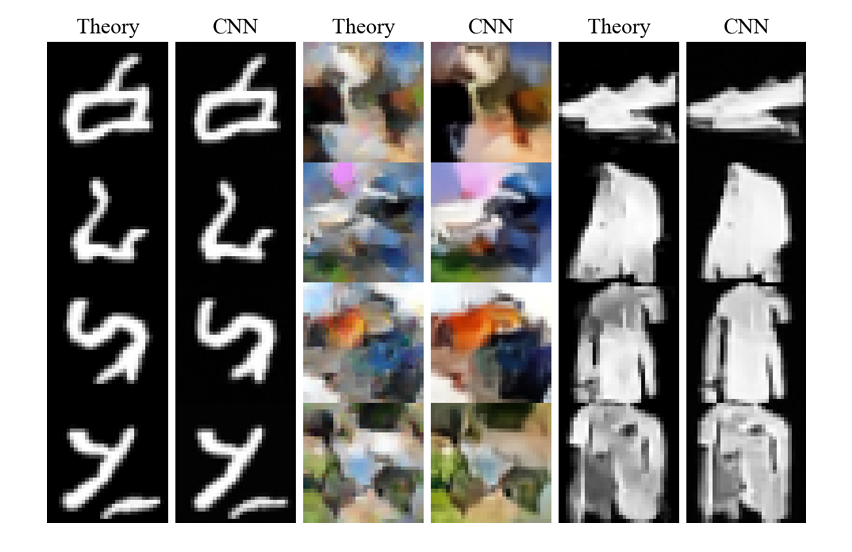
\includegraphics[width=0.5\textwidth]{../images/introduction_Ganguli.png} % Change width and filename
    \caption{Predicted images by analytic theory (left columns) and the output of convolutional diffusion model (right columns) (Source:\cite{kamb2024analytictheorycreativityconvolutional})}
    \label{fig:introduction_im}
\end{figure}

Our objective is to understand the mathematics involved in \cite{kamb2024analytictheorycreativityconvolutional} and to adapt them to address the resolution of inverse problems as well. The present study focuses on two key areas: diffusion-based generative models for image generation, inverse problems for recovery of original images from noisy measurements.

The paper is structured as follows. Section 2 introduces the core concepts underlying convolutional neural networks (CNNs), score-based diffusion models, and inverse problems, along with the empirical risk minimization framework. Section 3 analyzes analytical solutions for MMSE denoising  under different scenarios: no constraints, equivariance to a group of transforms, locality, and a mix between locality and equivariance. Section 4 presents preliminary research findings on MMSE inverse problems under  equivariance and/or locality constraints. Finally, Section 5 concludes with a discussion of implications and future research directions.

\section{Premilinairy}
\subsection{Convolutional neural network (CNN)}
Convolutional Neural Networks (CNNs) are a class of neural architectures defined as a succession of convolutions followed by nonlinear activation functions. 
In their simplest form, they can be written as:
\begin{equation*}
    N(x)  = \sigma\left( A_D \cdot \sigma \left( A_{D-1} \cdot \sigma \left( \hdots \sigma\left( A_1 \cdot x \right)\right)\right)\right),
\end{equation*}
where $\sigma: \R^N\to \R^N$ is a pointwise activation function (e.g. ReLU,  Sigmoid), $D\in \N$ denotes the depth of the network and $A_d : \R^{N\times w_d}\to \R^{N\times w_{d+1}}$ is a linear convolutional layer, that takes as an input a set of $w_d$ signals and outputs a set of $w_{d+1}$ signals with $w_1=w_{D+1} = 1$. Each operator $A_d$ is parameterized by convolution filters that constitute the weights of the networks. 
They are optimized for a particular task during the training phase. 
The layer $A_d$ takes the form:
\begin{equation}
    [A_d \cdot \{z_1,\hdots, z_{w_d}\}]_{j} = \sum_{i=1}^{w_d} h_{d,j,i} * z_i, 
\end{equation}
where $h_{d,j,i}$ are the convolution filters (the weights of the network) and $*$ denotes a discrete convolution. Throughout the paper we will assume that periodic boundary conditions are used. 

This specific structure induces two constraints on the network: locality and translation equivariance. 
By construction, if $x_\tau$ is a shifted version of $x$, $N(x_\tau)$ is nothing but $N(x)_{\tau}$, that is a shifted version of $N(x)$. 
This is the definition of translation equivariance.
Second, the locality is related to the fact that the convolution filters $h_{d,j,i}$ have a finite extent to reduce the number of parameters. 
Hence the value $N(x)$ at a certain location $t$ only depends on a patch of $x$ centered at $t$. 

CNNs are particularly well-suited for analyzing spatially structured data, such as images, physical fields, or spatiotemporal patterns, due to their ability to exploit the intrinsic structure and symmetries of such data. 

% \subsubsection{Translation Equivariance}
% The convolution operation inherently satisfies translation equivariance. This means that when an input is shifted, the output feature map shifts by the same amount, preserving spatial relationships. 
% The property of translation equivariance can be mathematically proved: given an input $x$, a filter $k$, we denote $y$ the convolution of $x$ and $k$:
% \begin{equation*}
%     y[m,n] = (x*k)[m,n] = \sum_{i,j} x[m-i,n-j]*k[i,j]
% \end{equation*}
% Let denote $z$ the shifted version of $x$ obtained by shifting $\delta_h$ pixels to the left and $\delta_v$ pixels to the bottom, i.e. $z[i,j] = x[i+\delta_h,j+\delta_v]$ the convolution of $z$ and $k$ follows:
% \begin{align*}
%     (z*k)[m,n] &= \sum_{i,j} z[m-i,n-j]*k[i,j]\\
%     &= \sum_{i,j} x[m-i+\delta_h,n-j+\delta_v]*k[i,j]\\
%     &= (x*k)[m+\delta_h,n+\delta_v]
% \end{align*} 
% \subsubsection{Locality}
% CNNs incorporate the principle of locality by using filters (kernels) of finite spatial extent. This means each computation depends only on a bounded region of the input, reflecting the assumption that meaningful patterns and interactions are primarily local.
\subsection{Diffusion Models}
Diffusion models generate data by learning to reverse a gradual noising process. In the forward process, clean data is progressively corrupted by adding noise in multiple steps until it becomes indistinguishable from random noise. In the reverse process, a neural network is trained to denoise the data step by step, effectively learning how to reconstruct the original samples. The two processes are illustrated by \Cref{fig:Diffusion_model}. In practice, this two-stage approach is highly effective for generating high-quality images, audio, and other complex data.
\begin{figure}[ht] % 'h' means 'here'
    \centering
    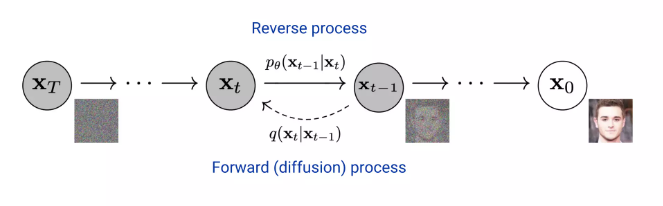
\includegraphics[width=0.5\textwidth]{../images/Diffusion_model.png} % Change width and filename
    \caption{Illustration of forward and reverse process \cite{slideshare2025}}
    \label{fig:Diffusion_model}
\end{figure}

\subsubsection{Notation conventions}
The notation used throughout the remainder of this work is as follows:
\begin{itemize}
    \item $\D$ represents the training set
    \item $x_0\in\R^N$ represents an example from the training set. For images of size L pixels by L pixels by C channels, we have $N=L\times L \times C$.
    \item For image data, $x[n]$ and $x_0[n]$ represent the pixel values of the images $x$ and $x_0$ at pixel location $n$; both are elements of $\R^C$.
    \item For a square image patch $b$ with an odd-dimension side length, the value $b[0] \in \R^C$ indicates the pixel at the center of the patch.
\end{itemize}
\subsubsection{Stochastic differential equations (SDE) and probability flows}

An important part of probabilistic modeling is to generate samples from a data distribution whose precise shape is unknown or too complex to allow direct sampling. Diffusion models offer a solution to this problem by learning a time-inhomogeneous differential equation, which gradually transforms samples from a simple Gaussian distribution into samples corresponding to the more complex target distribution.

Consider a time-dependent stochastic differential equation (Itô), given as follows:
    \begin{equation}\label{eq:SDE}
         dx_t = f_t(x_t)dt + g_tdW_t
    \end{equation}
    with 
    \begin{itemize}
        \item $x \in \mathbb{R}^N$
        \item $f_t \in C^1(\R^N,\R^N)$ and satisfies $\exists\, C > 0$ such that $\|f_t(x)\| \leq C(1 + \|x\|)$, where $\|\cdot\|$ denotes the $L^2$ norm, i.e., $\forall n \in \mathbb{N}^*, \forall x \in \mathbb{R}^n,\ \|x\| = \sqrt{\sum\limits_{i=1}^n x_i^2}$.
        \item $g_t$ is a $C^2$ function of $t$.
        \item $W_t$ is a standard Wiener process in $\mathbb{R}^N$, with
        \begin{equation*}
            \langle W^i, W^j \rangle_t =
            \begin{cases}
                t & \text{if } i = j \\
                0 & \text{otherwise}
            \end{cases}
        \end{equation*}
        where $W^i$ and $W^j$ are the $i$-th and $j$-th coordinates of $W_t$, respectively.
    \end{itemize}
    
    \begin{remark}
        The condition that $f_t$ is at most linearly increasing guarantees the existence of a SDE solution.
    \end{remark}

\begin{proposition}[Forward Process (Fokker – Planck)\label{prop:fokker}] 
    Under the above assumptions, the flow over the $\pi_t$ probability distributions of $x_t$ for $t \geq 0$ is given by :    \begin{equation}\label{eq:Fokker-Planck}
        \frac{\partial\pi_t}{\partial t} = -\nabla \cdot (f_t \pi_t) + \frac{1}{2}\nabla^2(g_t^2\pi_t)
    \end{equation}
\end{proposition}
\begin{proof}
    The proof is given in \Cref{sec:proof_focker}.
\end{proof}
% The condition that $f_t$ is at most linearly increasing guarantees the existence of an EDS solution.
% In general, the forward process is usually constructed so that as $t \rightarrow \infty$ (or $t \rightarrow T$ for some finite time $T$), the distribution $\pi_t$ converges to a known and well-defined distribution $\pi_{\infty}$, often chosen as the normal distribution.
In the context of diffusion models, and more specifically implicit diffusion models for denoising (DDIMs), the objective is to identify a deterministic, time-dependent vector field $v_t$ that exhibits the same flow of probability distributions as the preceding stochastic equation. This reformulation enables the diffusion process to be inverted deterministically:
\begin{itemize}
    \item We begin by sampling $x_T \sim \pi_t$
    \item Then we evolve the sample backwards in time, from $t=T$ to $t = 0$, by solving the following ODE:
    \begin{equation}
        \frac{dx_t}{dt} = v_t(x_t)
    \end{equation}
\end{itemize}
According to the Fokker-Planck equation, the evolution of the $x_t$ 's distribution is given by the following transport equation:
\begin{proposition}[reverse process\label{prop:fokker}] 
The reverse process is giving by the following equation
\[\frac{d\pi_t(x)}{dt} =-\nabla \cdot [v_t(x)\pi_t(x)]\]
\end{proposition}
\begin{proof}
    The above result is a direct application of \Cref{eq:Fokker-Planck}.
\end{proof}
Our goal is to identify the deterministic, time-dependent $v_t$ function so that the above equation produces the same evolution as \Cref{prop:fokker} (flow-matching). To do this, we rewrite \Cref{prop:fokker} as follows:
\[\frac{d\pi_t(x)}{dt} =\nabla \cdot([f_t(x)-\frac{1}{2}g_t^2\nabla \log\pi_t(x)]\pi_t(x))\]
Thus,
\[v_t(x) =f_t(x)-\frac{1}{2}g_t^2\nabla \log\pi_t(x) \]
We denote $s_t(x) \equiv \nabla \log\pi_t(x)$, $s_t$ is called a \emph{score function}. Determining this function plays an important role in recovering the initial image $x_0$.
\subsubsection{Flow calculation}\label{sec:calcul_numerique}
In practice, the most common choice of forward process for a DDIM is an inhomogeneous Ornstein-Uhlenbeck process. If a positive sequence $(\gamma_t)$  is chosen, it takes the following form:
\begin{equation}\label{eq:OU}
    dx_t = -\gamma_tx_t \,dt + \sqrt{2\gamma_t}\,dW_t
\end{equation}
By identifying in this case $f_t(x) = -\gamma_tx_t$ and $g_t = \sqrt{2\gamma_t}$, we deduce the expression for $v_t$ :
\begin{equation}\label{eq:backward}
    \frac{dx_t}{dt} = v_t(x_t) = -\gamma_t(x_t+\nabla \log \pi_t(x_t)) = -\gamma_t(x_t+s_t(x))
\end{equation}
% In this particular instance, it can be demonstrated that $f_t (x_t) = -\gamma_t x_t,  \text{ and } \mathcal{G}_t = \sqrt{2\gamma_t}$. Through these relationships, the expression for $v_t$ can be deduced:
% The expression $v_t (x_t)$ above defines a deterministic vector field, thereby enabling the diffusion process to be reversed by progressively eliminating the noise added during the direct phase. This field integrates the current position, denoted by the symbol $x_t$, and the score field, denoted by the symbol $s_t$, with the score field weighted by a factor $\gamma_t$. The integration of these two fields indicates the direction of maximum probability. In this manner, the quantity $v_t(x_t)$ functions as a guide for the evolution of $x_t$ in a continuous and reversible manner, thereby ensuring that the initially noisy sample $x_T$ is gradually transformed into the original domain data. This ordinary differential equation (ODE) reformulation is imperative for DDIM models, as it facilitates accelerated and optimized generation by circumventing the stochastic simulation of the inverse process.
The forward process given by \Cref{eq:OU} is chosen due to the fact that, for any $t \geq 0$, the solution $x_t$ is distributed according to a known distribution, as indicated by the following proposition:
\begin{proposition}\label{prop:solution_processus_direct}
    The solution $x_t$ of \Cref{eq:OU} is given by
    \begin{equation}\label{eq:solforphi}
        x_t = \sqrt{\bar{\alpha_t}}x_0 + \sqrt{1-\bar{\alpha_t}}\eta
    \end{equation}
    Where $x_0 \sim \pi_0$ is the distribution of the initial images to be sampled, $\eta$ is an isotropic Gaussian vector, i.e. $\eta \sim \mathcal{N}(0, I_N)$, and $\bar{\alpha_t}$ is defined by 
    \[\bar{\alpha_t} = \exp{\left(-2\int_0^t \gamma_s ds\right)}.\]    
\end{proposition}
\begin{proof}
    The proof is detailed in \Cref{sec:proof_solution_processus_direct}
\end{proof}
In particular, we implicitly choose $\gamma_t$ so that $\bar \alpha_t \rightarrow 0$ when t tends towards $T$. Therefore, the distribution $\pi_t$ tends to reduced-centered normal distribution and no longer depends on the initial  distribution $\pi_0$ as $t \rightarrow T$. The time-dependent parameter $\bar \alpha_t$ is called the “noise schedule”, as it controls the speed of convergence $\pi_t$. We can therefore sample $x_T$ a centered reduced normal distribution, then recover $x_0$ by using the reverse process.

% The fundamental premise of the diffusion model hinges on the reversal of the forward process, thereby facilitating the sampling of the target distribution, denoted by $p_0$, through the inverse process. The latter requires knowledge of the score function $s_t = -d/dlog(p_t)$. The initial step in this process is the calculation of the probability distribution of the random variable $x_t$, denoted by $\pi_t$.

% The following two results are essentially useful for calculating the analytical expression of $\pi_t$.
% \begin{proposition}\label{prop:quelques_resultats_sur_la_densite}
%     Let X and Y be two independent random variables in $\R^n$, $f_X$ and $f_Y$ are the density functions of $X$ and $Y$ respectively. We obtain the following properties:
% \begin{enumerate}[label=(\roman*)]
%     \item[] Let $\alpha \in \R_+^*$, and $U = \alpha X$, then the density fonction of $U$ is given by $\forall x\in \R^n$, $f_U(x) = \frac{1}{\alpha^n} f_X(\frac{x}{\alpha})$.
%     \item[] Let $Z = X+Y$, The density of $Z$ is the convolution of the the density funciton of $X$ and the density function of $Y$, i.e. $f_Z(x) = (f_X * f_Y)(x)$
% \end{enumerate}
% \end{proposition}

% \begin{proof}
% The proof of these results is detailed in \Cref{sec:proof_quelques_resultates_sur_la_densite}.
% \end{proof}


% The objective is to express the density of the target state, denoted by the symbol $\pi_t$, in terms of the transformations undergone by the probe state, denoted by the symbol $x_t$, during the forward process. Two above results on the densities of random variables are employed: firstly, the linear transformation of a random variable, which enables the deduction of the effect of a scaling factor on the density; and secondly, the convolution of densities, which facilitates the calculation of the density of the sum of two independent random variables. By employing the aforementioned properties, it is possible to express the probability of the occurrence of the phenomenon under consideration, denoted here by $\pi_t$, as an integral of the initial density $\pi_0$, convolved with a normal distribution of covariance \((1 - \bar{\alpha}_t) I_N\). This reflects the progressive diffusion of the initial distribution under the effect of Gaussian noise. To be more precise, the distribution of the random variable $t$ is given by the following proposition.
\begin{proposition}\label{prop:distribution_a_etap_t}
    Let the forward process presented by \Cref{eq:solforphi}, under the assumption of the existence of the $\pi_t$ distribution of $x_t$, The distribution $\pi_t$ is given by:    
    \begin{equation}\label{eq:distribution_pi_t}
        \pi_t(x) = \int_{\R^N} \pi_0(z)\, \mathcal{G}_t(x - \sqrt{\bar \alpha_t}\,z) dz
    \end{equation}
    with $\mathcal{G}_t$ the density function of a normal distribution $\mathcal{N}\left(0_{\R^N}, (1- \bar\alpha _t \,)I_N\right)$
\end{proposition}

\begin{proof}
    See \Cref{sec:proof_distribution_a_etap_t} for the full proof.
\end{proof}
% The analytical expression of $\pi_t$ shows that the forward process applies a progressive smoothing to the initial distribution $\pi_0$, convolving it with a normal distribution. Under the assumption that $\bar \alpha_t \rightarrow \infty$ when $t$ tends towards $1$ (or towards some large $T$), the larger $t$ is, the further $x_t$ is from its initial state and tends towards an isotropic normal distribution.
We derive the score function from $\pi_t$ :
\begin{align*}
        s_t(x) &= \nabla \log \pi_t(x) = \frac{1}{\pi_t(x)}\nabla\pi_t(x) \\
        &= \frac{1}{\pi_t(x)}\nabla\int_{\R^N} \pi_0(z) g(x - \sqrt{\bar \alpha_t} \,z) dz\\
\end{align*}
Let's denote $u: \R^N \times \R^N \rightarrow \R$ the quantity inside the above integral defined by:
\[u(x,z) =  \pi_0(z) \mathcal{G}_t(x - \sqrt{\bar \alpha_t}\,z), \quad \forall (x,z) \in \R^N \times \R^N\]
The function $u$ is continuous on $\R^N \times \R^N$ and integrable with respect to $z$. Furthermore, $\nabla_x u$ exists, is continuous on $\R^N \times \R^N$ and is integrable with respect to $z$. Then, using Leibniz's integral rule, we obtain :
\begin{equation}\label{eq:score_formule_premilinaire}
    s_t(x) = \frac{1}{\pi_t(x)} \int_{\R^N} \pi_0(z) \nabla_x \mathcal{G}_t(x - \sqrt{\bar \alpha_t} \,z) dz 
\end{equation}
Since $\mathcal{G}_t$ is the normal law density function $\mathcal{N}\left(0_{\R^N}, (1-\sqrt{\bar \alpha _t},)I_N\right)$, by definition, the function $\mathcal{G}_t$ is written :
\begin{equation*}
    \mathcal{G}_t(x) = \frac{1}{\sqrt{2\pi}(1-\bar \alpha_t)^{\frac{N}{2}}} \, \exp\left(-\frac{1}{2(1-\bar \alpha _t)}\,x^Tx\right) \quad \forall x \in \R^N
\end{equation*}
Thus
\begin{equation*}
    \nabla_x \,\mathcal{G}_t(x) = -\frac{1}{1-\bar \alpha_t}g(x)x
\end{equation*}
Thus
\begin{equation*}
    \nabla_x \,\mathcal{G}_t(x - \sqrt{\bar \alpha_t} \,z) = -\frac{1}{1-\bar \alpha_t}\,\mathcal{G}_t(x - \sqrt{\bar \alpha_t} \,z)(x - \sqrt{\bar \alpha_t} \,z)
\end{equation*}
Substituting this result into \Cref{eq:score_formule_premilinaire} :
\begin{equation}\label{eq:score_formule_analytique}
    s_t(x) = -\frac{1}{1- \bar \alpha_t} \int_{\R^N} \frac{\pi_0(z)\, (x - \sqrt{\bar \alpha_t} \,z) \mathcal{G}_t(x - \sqrt{\bar \alpha_t} \,z)}{\pi_t(x)} dz
\end{equation}
% The equation \Cref{eq:score_formule_analytique} expresses the score function \(s_t\), which represents the logarithmic gradient of the density \(\pi_t\). This function indicates the direction in which \(\pi_t\) must be adjusted to recover a probable initial state. The integral shows that \(s_t(x)\) is obtained by averaging over all possible initial values \(z\), weighted by their original probability \(\pi_0(z)\) and the noise added during diffusion. The term \((x - \sqrt{\bar{\alpha}_t}\, z)\) reflects the correction needed to reverse the diffusion, and normalization by \(\pi_t(x)\) ensures that this correction is local. Finally, the factor \(-\frac{1}{1- \bar \alpha_t}\) adjusts the intensity of this correction according to the noise level. This result is fundamental to scattering models, as it enables us to estimate the optimal direction in which to remove the added noise, thus generating realistic samples from initial noise.
The intervention of the target distribution $\pi_0$ makes the score function $s_t$ implicit. However, this score function can be learned from the data by using the Tweedie's formula.
\begin{theorem}[Tweedie's formula]\label{theo:formule_de_Tweedie}
    Let $X \in \mathbb{R}^n$ be a random variable of density $f_X$ and $B \sim \mathcal{N}(0, \sigma^2 I_n)$ a Gaussian noise independent of $X$. We define :
    \[ Y = X + B \]
    Let's denote $\varphi_B$ and $p_Y$ the density function of $B$ and $Y$ respectively. We obtain :
    \[ \mathbb{E}[X | Y = y] = y + \sigma^2 \nabla \log p_Y(y) \]
\end{theorem}
\begin{proof}
    The proof given in \Cref{sec:proof_formule_de_Tweedie}
\end{proof}
We recall the forward process
\[ x_t = \sqrt{\bar \alpha_t} x_0 + \sqrt{1 - \bar \alpha_t} \eta \]
Using the  Tweedie formula, we derive the score function :
\begin{align*}
s_t(x) &= \nabla \log \pi_t(x) \\
&= \frac{-x + \mathbb{E} \left[\sqrt{\bar \alpha_t}\, x_0 \mid x_t = x \right]}{1 - \bar \alpha_t} \\
&= \frac{1}{1 - \bar \alpha_t} \left( -x + \sqrt{\bar \alpha_t} \,\mathbb{E} \left[ x_0 \mid x_t = x \right] \right)
\end{align*}
The above result is extremely useful, allowing us to numerically approximate the score function $s_t$, which is proportional to $\mathbb{E}[x_0 | x_t]$. which is the orthogonal projection of $x_0$ onto the functional space of $x_t$, i.e. 
\[
\mathbb{E}[x_0 | x_t] = \argmin_{f \in \mathbb{L}^2(\mathbb{R}^N)} \mathbb{E}\left[ \| x_0 - f(x_t) \|^2 \right], \quad t \in [0,T]
\]
Therefore, learning the score function is equivalent to finding an MMSE estimator of $x_0$. Theoretically, the learned function is found by minimizing the above MSE regression on $L_2(\R^N)$. However, in the context of convolutional diffusion models, the learned function is constrained to be local and translation equivariant due to the architectural nature of convolutional neural networks, motivating us to analytically describe the behavior of CNN outputs.

% Ainsi, la fonction de score $s_t = \frac{-1}{(\alpha_t)^{N/2} \sqrt{1-\bar{\alpha}_t}} \mathbb{E}\left[ \eta - f(x_t) \right]$ est définie comme :
% \[
% s_t = \argmin_{f \in \mathbb{L}^2(\mathbb{R}^N)} \mathbb{E}\left[ \left\| \frac{1}{(\bar \alpha_t)^{N/2} \sqrt{1-\bar{\alpha}_t}} \eta + f(x_t) \right\|_2^2 \right], \quad t \in [0,T]
% \]
% We want to approximate $s_t$ for all $t \in [0,T]$, not just on a given $t$. This idea motivates us to build a neural network that models a function $f_z(x,t)$ by minimizing the following cost function:
% \[
% \mathcal{L}(z) = \mathbb{E}_{t \sim U([0,T]), x_t \sim \pi_t, x_0 \sim \pi_0} \left[ \| f_z(x_t,t) - x_ 0\|^2 \right]
% \]
% The optimal function $f_z$ can be approximated numerically by solving the associated regression problem. Once $f_z$ has been acquired, the score function $s_t$ can be obtained directly by :
% \[
% s_t(x)= \frac{1}{1 - \bar \alpha_t} \left( -x + \sqrt{\bar \alpha_t} \, f_z(x,t) \right)
% \]

\subsection{Inverse Problem}
Inverse problems aim to recover a target variable $x \in \R^N$ from a noisy measure $y \in \R^M$, typically modeled as
\begin{equation*}
    y = Ax +b, \text{ with } A:\R^N \rightarrow \R^M
\end{equation*}
An approach is to learn a function $f : y \rightarrow \hat{x}$ using a convolutional neural network trained on a supervised dataset ${(x_i,y_i)}_{i=1}^\mathcal{D}$. The network is trained by minimizing the empirical risk associated with a loss function
\begin{equation*}
    \argmin_{f\in \mathcal{F}_{\text{CNN}}} \E{\norm{f(y)-x}}
\end{equation*}
where $\mathcal{F}_{\text{CNN}}$ denotes the admissible set of functions expressible by the chosen CNN architecture. This restriction imposes structural constraints such as locality and translation equivariance.


    

\subsection{Conclusion}
In the context of both diffusion models and inverse problems, uderstanding how a neural network works requires us to analyze MMSE estimator. Surprisingly, the locality and equivariance constraints alone are sufficient to predict the network's behavior \cite{kamb2024analytictheorycreativityconvolutional}.

\section{Analytical solution for the MMSE denoising}
The MMSE denoising problem corresponds to a special case of the inverse problem where the forward operator is the identity, i.e., $A = \mathrm{Id}$. This is precisely the setting studied in Ganguli et al. (2024) \cite{kamb2024analytictheorycreativityconvolutional}. In this section, our objective is to understand and reconstruct the main theoretical results presented in their work in order to better understand the behavior and expressivity of convolutional denoising networks.
\subsection{Ideal Score (IS) machine}
We show in this section that a diffusion model that learns the ideal score function, i.e. without any constraints, on a finite dataset can only memorize and cannot create new samples that are different from the training data.

We do not have access to the target distribution $\pi_0$ because we have a finite number of samples, so we estimate it by the empirical discrete distribution on the training data set $\mathcal{D}$ :
\begin{equation*}
    \pi_0(x) = \frac{1}{|\mathcal{D}|} \sum\limits_{x_0  \in \mathcal{D}} \delta(x - \varphi)
\end{equation*}
With $|\mathcal{D}|$ the number of elements in $\mathcal{D}$ and $\delta$ a Dirac mass. By using \Cref{eq:distribution_pi_t}, At temporal step $t$, we obtain the distribution of noised images :
\begin{align*}
\pi_t(x) &= \int_{\mathbb{R}^N} \pi_0(z) \mathcal{G}_t(x - \sqrt{\bar \alpha_t}z) dz \quad \text{with } \mathcal{G}_t \text{ is the density function of normal distribution } \mathcal{N}(0, (1-\bar \alpha_t)I_N) \\
&= \frac{1}{|\mathcal{D}|} \sum\limits_{x_0  \in \mathcal{D}} \int_{\mathbb{R}^N} \delta(z - x_0) \mathcal{G}_t(x - \sqrt{\bar \alpha_t}z) dz \\
&= \frac{1}{|\mathcal{D}|} \sum\limits_{x_0  \in \mathcal{D}} \mathcal{G}_t(x - \sqrt{\bar \alpha_t}x_0)
\end{align*}

The estimated score function $s_t = \nabla \log \pi_t$, which gives us 
:\begin{align*}
s_t(x) &= \nabla \log \pi_t(x) = -\sum\limits_{x_0  \in \mathcal{D}} (x - \sqrt{\bar \alpha_t}x_0) \frac{\mathcal{G}_t(x - \sqrt{\bar \alpha_t}x_0)}{\pi_t(x)} \\
&= -\frac{1}{1-\bar \alpha_t} \sum\limits_{x_0  \in \mathcal{D}} (x - \sqrt{\bar \alpha_t}x_0) W_t(x_0 | x) \\
& \text{with }W_t(x_0| x) = \frac{\mathcal{G}_t(x - \sqrt{ \bar \alpha_t}x_0)}{\sum\limits_{x_0'  \in \mathcal{D}} \mathcal{G}_t(x - \sqrt{\bar \alpha_t}x_0')}
\end{align*}

% \begin{align*}
% s_t(x) &= -\frac{1}{1-\bar \alpha_t} \,\frac{\sum\limits_{x_0  \in \mathcal{D}} (x - \sqrt{\bar \alpha_t}x_0) \mathcal{G}_t(x - \sqrt{ \bar \alpha_t}x_0)}{\sum\limits_{x_0'  \in \mathcal{D}} \mathcal{G}_t(x - \sqrt{\bar \alpha_t}x_0')}
% \end{align*}
% In general, this process involves averaging the added noise. This is done by taking the noise vectors $\eta \propto (x - \sqrt{\bar \alpha_t}x_0)$ between the observed example $x$ and each training element $\varphi$, with weights based on the probability $W(\varphi|x)$ that the noisy image $x_t$ at time step $t$ would come from a point $\varphi$ of the training set $\mathcal{D}$ . This probability is calculated using Bayes' theorem: it is the probability that a training example $\varphi$ will give the observed example $x$, as a function of the amount of noise required to transform $\varphi$ into $x$, compared with all other possible examples $\varphi'$. The weights $W(\varphi|x)$ are calculated using a simple softmax function applied to a quadratic loss function $-\frac{1}{2(1-\bar \alpha_t)}\||x - \sqrt{\bar \alpha_t}x_0|^2$ for each $\varphi$ point in the training set.
Our aim is to show that $x_t$ converge to an element $x_0 \in \mathcal{D}$ as $t \rightarrow 0$. We first recall the reverse process:
\begin{equation*}
    \frac{dx}{dt} =  -\gamma_t(x+s_t(x)), \quad \text{avec } \gamma_t = -\frac{\partial \bar \alpha_t}{2\bar \alpha_t} 
\end{equation*}
% Lors du processus inverse, le score idéal agit comme un guide dynamique : il calcule, pour chaque sample \(x_t\), des forces proportionnelles à la proximité de \(x_t\) avec chaque donnée atténuée $\sqrt{\bar \alpha_t} \varphi$, pondérées par des probabilités \emph{a posteriori} (\(W_t(\varphi|x)\)). Ce score crée un effet d’amplification : si le sample est proche d’une donnée réduite, le modèle devient plus "sûr" que c’est la bonne direction, et le tire encore plus vers elle. Cette certitude augmente progressivement, forçant le sample à converger vers exactement la même donnée d’entraînement.
% Il est important de noter que la fonction de score idéale ne correspond pas vraiment aux modèles de diffusion réels. Elle a tendance à mémoriser les données d'entraînement, surtout lorsqu'on travaille avec des données à haute dimension, car les points d'entraînement sont très éloignés les uns des autres. Cela nécessite beaucoup plus de données pour bien couvrir l'espace sous-jacent afin que la fonction de score empirique puisse bien approximer la vraie fonction de score idéale pour toutes les entrées et à tous les moments.
% Le fait que la fonction de score idéale ne soit pas un bon modèle pour les processus de diffusion réalistes nous montre qu'il faut comprendre pourquoi ces modèles ne résolvent pas parfaitement leurs tâches. Il faut donc examiner les biais et contraintes qui empêchent ces modèles d'apprendre la fonction de score idéale et voir comment ils se comportent malgré ces limitations.
Assume that the limits \( \lim_{t \to 0} x_t \) and \( \lim_{t \to 0} \partial_t x_t \) exist, which implies that
\[
\lim_{t \to 0} \gamma_t s_t(x_t) \text{ also exist.}
\]
We have
\begin{equation*}
    \lim\limits_{t \to 0} \gamma_t s_t (x_t) = \lim\limits_{t \to 0} \frac{\partial \bar{\alpha}_t}{2\bar{\alpha}_t} \frac{1}{1 - \bar{\alpha}_t} \sum\limits_{x_0 \in \mathcal{D}} \left( x_t - \sqrt{\bar{\alpha}_t} x_0 \right) W(x_0 | x_t)
\end{equation*}
As  $\lim\limits_{t \to 0} \bar{\alpha}_t = 1$, the prefactor diverges. This means:
\begin{equation*}
    \lim\limits_{t \to 0} \sum\limits_{x_0 \in D} (x_t - \sqrt{\bar{\alpha}_t} x_0) W(x_0 | x_t) = 0
\end{equation*}
We note that $\mathcal{N}(x_t | \sqrt{\bar{\alpha}_t} x_0, (1 - \bar{\alpha}_t) I_N)$ tends towards a dirac function when $t \to 0$ because $\bar{\alpha}_t \xrightarrow[]{t \to 0} 1$ . Thus
\begin{equation*}
    \lim\limits_{t \to 0} W(x_0 | x_t) =
\begin{cases} 
1 & \text{if } x_0 = x_0^* \coloneq \arg\min_{x_0 \in D} ||x_t - x_0||^2 \\
0 & \text{else}
\end{cases}
\end{equation*}
% Indeed
% \begin{equation*}
%     W(x_0 | x_t) =
% \frac{\exp\left( -\frac{||x_t - \sqrt{\bar{\alpha}_t} x_0||^2}{(1 - \bar{\alpha}_t)^N} \right)}
% {\sum\limits_{x_0' \in D} \exp\left( -\frac{||x_t - \sqrt{\bar{\alpha}_t} x_0'||^2}{(1 - \bar{\alpha}_t)^N} \right)}
% =\frac{1}{\sum\limits_{x_0' \in D} \exp\left( \frac{||x_t - \sqrt{\bar{\alpha}_t} x_0'||^2 - ||x_t - \sqrt{\bar{\alpha}_t} x_0||^2}{(1 - \bar{\alpha}_t)^N} \right)}
% \end{equation*}
% Let $A(x_t, x_0, x_0' ) = \exp\left( \frac{||x_t - \sqrt{\bar{\alpha}_t} x_0'||^2 - ||x_t - \sqrt{\bar{\alpha}_t} x_0||^2}{(1 - \bar{\alpha}_t)^N} \right)$, we note that
% \begin{equation*}
%     \lim\limits_{t \to 0} A(x_t, x_0, x_0^*) =
% \begin{cases} 
% +\infty & \text{if } x_0 \neq x_0^* \\
% 1 & \text{if } x_0 = x_0^*
% \end{cases}
% \end{equation*}
% In addition
% \begin{equation*}
%     \lim\limits_{t \to 0} A(x_t, x_0^*, x_0') = 0 \quad \forall x_0' \in D \setminus \{x_0^*\}
% \end{equation*}
% Thus
% \[
% \lim\limits_{t \to 0} W(x_0 | x_t) =
% \begin{cases} 
% 1 & \text{if } x_0 = x_0^* \\
% 0 & \text{else}
% \end{cases}
% \]
We obtain
\[
0 = \lim\limits_{t \to 0} \sum\limits_{x_0 \in D} (x_t - \sqrt{\bar{\alpha}_t} x_0) W(x_0 | x_t) = \lim\limits_{t \to 0} (x_t - x_0^*)
\]
\begin{equation*}
    \lim\limits_{t\rightarrow 0} x_t = x_0^* \in \mathcal{D}
\end{equation*}

In conclusion, at date $t = 0$, the sample tends towards an image in the training set $\mathcal{D}$. However, the ideal score function does not accurately capture the behavior of real-world diffusion models, showing us that we need to understand why these models don't solve their tasks perfectly. We therefore need to examine the biases and constraints that prevent these models from learning the ideal score function, and see how they perform despite these limitations.
\subsection{Score function estimator under constraints}
\subsubsection{General}
We would like to solve
\begin{equation*}
    \min_{f\in\mathcal{M}} \E{\| f(t,x)-s_t(x)\|}
\end{equation*}
for some vector space $\mathcal{M}$\\
$f^* \in \mathcal{M}$ is a minimiser of $J$ if $J(f^*+\epsilon h) \geq J(f^*)$ for all $\epsilon \in \R$ and all $h\in \mathcal{M}$. We have
\begin{align*}
    J(f^*+\epsilon h) &= \E{\|(f^*+\epsilon h)(t,x)-s_t(x)\|^2}\\
    & = J(f^*)+\epsilon^2\E{\|h(t,x)\|^2}+2\epsilon\E{\langle h(t,x),f*(t,x) - s_t(x) \rangle}
\end{align*}
therefore, the optimality condition follows
\begin{equation}\label{eq:optimal_condition_score_function}
    \E{\langle h(t,x),f*(t,x) - s_t(x) \rangle} = 0 \text{ for all } x \in \mathcal{M}
\end{equation}

\subsubsection{Equivariant score (ES) machine}
\begin{definition}[Group of transformation]
    A \textbf{group of transformations} is a set \( G \) of applications of a set \( X \) into itself, with a composition operation of transformations that satisfies the following axioms:
    \begin{itemize}[topsep=-5pt]
    \item[] \textbf{Closedness} : \( \forall U, V \in G, \quad U \circ V \in G \).
    \item[] \textbf{Associativity} : \( (U \circ V) \circ W = U \circ (V \circ W) \).
    \item[] \textbf{Identity} : \( \exists e \in G \) so that \( e \circ U = U \circ e = U \).
    \item[] \textbf{Inverse} : \( \forall U \in G, \quad \exists \,U^{-1} \in G \text{ tel que } U \circ U^{-1} = U^{-1} \circ U = e \).
\end{itemize}
\end{definition}



% For example, the symmetry group in $\R^2$ is the set of transformations that preserve the Euclidean distance. More precisely, it includes rotation and reflection:
% \begin{itemize}
%     \item[] A rotation of angle $z$ about the origin is given by the rotation matrix :\[
% R_z =
% \begin{bmatrix}
% \cos z & -\sin z \\
% \sin z & \cos z
% \end{bmatrix}.
% \]

% \item[] a reflection about any axis in \( \mathbb{R}^2 \) can be represented by a matrix of the form :
% \[
% S_\varphi =
% \begin{bmatrix}
% \cos \varphi & \sin \varphi \\
% \sin \varphi & -\cos \varphi
% \end{bmatrix}.
% \]
% This retains the standard, but reverses the direction.
% \end{itemize}

\begin{definition}
    A transformation group $G$ acting on a complex vector space $X$ provided with the scalar product $\langle \cdot,\cdot \rangle$ is said to be unitary if for any transformation $U \in G$, we have :
    \begin{equation*}
        \langle Ux,Uy\rangle = \langle x,y\rangle \quad\forall(x,y) \in X^2
    \end{equation*}
\end{definition}


% Transformations in a unitary group preserve geometric properties such as distances and angles between vectors, but only in complex vector spaces. The example of the $\R^2$ symmetry group above is also a unitary group.
% \begin{proposition}\label{prop:Groupe_unitaire}
%     Let G be a group of unitary transformations acting on a complex vector space X. Let $U$ be an element in $G$, and we have the following properties:
%         \begin{enumerate}[label=(\roman*)]
%         \item[] \textbf{Inverse et adjoint} : $\forall U \in G$, $U^{-1} = U^\dagger$ with $U^\dagger$ adjoint operateur of $U$.
%         \item[] \textbf{Préservation de norme} : $\|Ux\| = \|x\| \quad \forall x\in X$.
%         \item[] \textbf{Transformation de gradient} : for any $f \in C^1(X,\R)$, for any $x \in X$:
%         \begin{equation*}
%             \nabla_x f(U^{-1}x) = U\, \nabla f(U^{-1}x) \quad \forall x\in X.
%         \end{equation*}
%     \end{enumerate}
% \end{proposition}

% \begin{proof}
%     The proof is in \Cref{sec:proof_groupe_unitaire}
% \end{proof}
% L'équivariance dans les modèles de diffusion garantit que le processus génératif respecte les symétries naturelles des données, ce qui est essentiel pour de nombreuses applications. En intégrant ces symétries dans l'architecture du modèle, on préserve la cohérence structurelle des échantillons générés, tout en réduisant la redondance dans l'apprentissage et en améliorant la généralisation. Cela permet également une optimisation plus stable et évite l’introduction de dépendances arbitraires qui pourraient nuire à la performance du modèle. On va étudier dans cette section comment un modèle de diffusion apprend la fonction de score sous la contrainte d'équivariance.
The admissible set of function $\mathcal{M}$ is defined by
\begin{equation*}
    \mathcal{M} = \{f:[0,T]\times \R^N \rightarrow \R^N \text{ such that } f(t,T_g x) = T_g f(t,x), \quad \forall T_    g\in G,\forall x\in \R^N \}
\end{equation*}


We recall the optimal condition \Cref{eq:optimal_condition_score_function}
\begin{equation*}
\E{\langle h(t,x),f^*(t,x) -s_t(x)\rangle} = 0, \text{ for any } h \in \mathcal{M}
\end{equation*}
We have
\begin{align*}
    & \E{\langle h(t,x),f^*(t,x) -s_t(x)\rangle} \\
    &= \frac{1}{|\mathcal{D}|}\sum_{x_0  \in \mathcal{D}} \int_{\R^N} \langle h(t,x),f^*(t,x)-s_t(x) \rangle \mathcal{G}_t(x -\sqrt{\bar \alpha_t}x_0)dx\\
    &= \frac{1}{|\mathcal{D}|}\sum_{x_0  \in \mathcal{D}} \int_{\R^N} \int_{G }\langle h(t,x),f^*(t,x) \mathcal{G}_t(x -\sqrt{\bar \alpha_t}x_0)-s_t(x) \mathcal{G}_t(x -\sqrt{\bar \alpha_t}x_0) \rangle dx\\
    &= \frac{1}{|\mathcal{D}|} \int_{\R^N} \int_G \left\langle h(t,x),\sum_{x_0  \in \mathcal{D}}f^*(t,x) \mathcal{G}_t(x -\sqrt{\bar \alpha_t}x_0)-\sum_{x_0  \in \mathcal{D}} \frac{-1}{1-\bar \alpha_t} (x -\sqrt{\bar \alpha_t})\mathcal{G}_t(x -\sqrt{\bar \alpha_t}x_0)  \right\rangle dx\\
    &= \frac{1}{|\mathcal{D}|} \int_{\R^N} \int_G  \left\langle h(t,x),\sum_{x_0  \in \mathcal{D}}f^*(t,x) \mathcal{G}_t(T_g(x -\sqrt{\bar \alpha_t}x_0))-\sum_{x_0  \in \mathcal{D}} \frac{-1}{1-\bar \alpha_t} (x -\sqrt{\bar \alpha_t})\mathcal{G}_t(T_g(x -\sqrt{\bar \alpha_t}x_0))  \right\rangle dx dT_g\\
    &= \frac{1}{|\mathcal{D}|} \int_{\R^N} \int_G\Big\langle h(t,x),\sum_{x_0  \in \mathcal{D}}f^*(t,x) \mathcal{N}(T_gx,T_g \sqrt{\bar \alpha_t}x_0,(1-\bar\alpha_t)I_N) \\
    & \hspace{3cm}  - \sum_{x_0  \in \mathcal{D}} \frac{-1}{1-\bar \alpha_t} (x -\sqrt{\bar \alpha_t})\mathcal{N}(T_gx,T_g \sqrt{\bar \alpha_t}x_0,(1-\bar\alpha_t)I_N)  \Big\rangle dx dT_g\\
    &= \frac{1}{|\mathcal{D}|} \int_{\R^N} \int_G \Big\langle T_g^{-1}h(t,T_gx),\sum_{x_0  \in \mathcal{D}}T_g^{-1}f^*(t,T_gx) \mathcal{N}(T_gx,T_g \sqrt{\bar \alpha_t}x_0,(1-\bar\alpha_t)I_N)\\
    & \hspace{3cm} -\sum_{x_0  \in \mathcal{D}} \frac{-1}{1-\bar \alpha_t} T_g^{-1}(T_gx -T_g \sqrt{\bar \alpha_t}x_0)\mathcal{N}(T_gx,T_g \sqrt{\bar \alpha_t}x_0,(1-\bar\alpha_t)I_N)  \Big\rangle dx dT_g\\
    &= \frac{1}{|\mathcal{D}|} \int_{\R^N} \int_G \Big\langle T_g^{-1}h(t,T_gx),\sum_{x_0  \in \mathcal{D}}T_g^{-1}f^*(t,T_gx) \mathcal{N}(T_gx,T_g \sqrt{\bar \alpha_t}x_0,(1-\bar\alpha_t)I_N)\\
    & \hspace{3cm} -\sum_{x_0  \in \mathcal{D}} \frac{-1}{1-\bar \alpha_t} T_g^{-1}(T_gx -T_g \sqrt{\bar \alpha_t}x_0)\mathcal{N}(T_gx,T_g \sqrt{\bar \alpha_t}x_0,(1-\bar\alpha_t)I_N)  \Big\rangle dx dT_g\\
    &= \frac{1}{|\mathcal{D}|} \int_{\R^N} \int_G\Big\langle h(t,T_gx),\sum_{x_0  \in \mathcal{D}}f^*(t,T_gx) \mathcal{N}(T_gx,T_g \sqrt{\bar \alpha_t}x_0,(1-\bar\alpha_t)I_N)\\
    & \hspace{3cm}-\sum_{x_0  \in \mathcal{D}} \frac{-1}{1-\bar \alpha_t} (T_gx -T_g \sqrt{\bar \alpha_t}x_0)\mathcal{N}(T_gx,T_g \sqrt{\bar \alpha_t}x_0,(1-\bar\alpha_t)I_N)  \Big\rangle dx dT_g\\
    &= \frac{1}{|\mathcal{D}|} \int_{\R^N} \int_G\Big\langle h(t,x),\sum_{x_0  \in \mathcal{D}}f^*(t,x) \mathcal{N}(x,T_g \sqrt{\bar \alpha_t}x_0,(1-\bar\alpha_t)I_N)\\
    & \hspace{3cm}-\sum_{x_0  \in \mathcal{D}} \frac{-1}{1-\bar \alpha_t} (x -T_g \sqrt{\bar \alpha_t}x_0)\mathcal{N}(x,T_g \sqrt{\bar \alpha_t}x_0,(1-\bar\alpha_t)I_N)  \Big\rangle dx dT_g\\
    &= \frac{1}{|\mathcal{D}|} \int_{\R^N}  \Big\langle h(t,x),\int_G \sum_{x_0  \in \mathcal{D}}f^*(t,x) \mathcal{N}(x,T_g \sqrt{\bar \alpha_t}x_0,(1-\bar\alpha_t)I_N)\\
    & \hspace{3cm}-\sum_{x_0  \in \mathcal{D}} \frac{-1}{1-\bar \alpha_t} \int_G(x -T_g \sqrt{\bar \alpha_t}x_0)\mathcal{N}(x,T_g \sqrt{\bar \alpha_t}x_0,(1-\bar\alpha_t)I_N) \Big\rangle dx dT_g\\
\end{align*}
The optimality condition implies that the above quantity is zero $\forall h \in \mathcal{M}$, thus
\begin{equation*}
    \sum_{x_0  \in \mathcal{D}}\int_G f^*(t,x) \mathcal{N}(x,T_g \sqrt{\bar \alpha_t}x_0,(1-\bar\alpha_t)I_N)dT_g-\sum_{x_0  \in \mathcal{D}} \int_G \frac{-1}{1-\bar \alpha_t} (x -T_g \sqrt{\bar \alpha_t}x_0)\mathcal{N}(x,T_g \sqrt{\bar \alpha_t}x_0,(1-\bar\alpha_t)I_N)dT_g  =0
\end{equation*}
Thus
\begin{equation*}
    f^*(t,x) =\frac{-1}{1-\bar \alpha_t}\frac{\sum_{x_0  \in \mathcal{D}}\int_G  (x -T_g \sqrt{\bar \alpha_t}x_0)\mathcal{N}(x,T_g \sqrt{\bar \alpha_t}x_0,(1-\bar\alpha_t)I_N) dT_g}{\sum_{x_0  \in \mathcal{D}}\int_G \mathcal{N}(x,T_g \sqrt{\bar \alpha_t}x_0,(1-\bar\alpha_t)I_N) d T_g}
\end{equation*}
% The conditions on the transformation $T_g$ are important: We need to do a change of variable $T_g x \rightarrow x$ and pass the adjoint $T_g^{-1}$ to the other side of the inner product. The following properties were used:
% \begin{itemize}
%     \item[] $|\det(T_g T_g^\top)| = 1$
%     \item[] $(T_g^{-1})^\top=T_g $
% \end{itemize}
In the image case, $G$ corresponds to every possible spatial translation, which is indeed a group of unitary transformations. We also note that $G(\mathcal{D})$ is finite, since $\mathcal{D}$ contains a finite number of images and each image has a finite number of pixels. Consequently, integrals over $G$ in the above expression convert to sums over $G(\varphi)$ 
\begin{align*}
        f^*(t,x) &= -\frac{1}{1-\bar \alpha_t} \sum\limits_{x_0  \in \mathcal{D}} \sum\limits_{x_0' \in G(x_0)} (x - \sqrt{\bar \alpha_t} x_0') \frac{\mathcal{N}(x;\sqrt{\bar \alpha_t} x_0', (1-\bar \alpha_t) I_N) }{\sum\limits_{x_0  \in \mathcal{D}} \sum\limits_{x_0'\in G(\varphi)} \mathcal{N}(x;\sqrt{\bar \alpha_t} x_0', (1-\bar \alpha_t) I_N)}\\
        &= -\frac{1}{1-\bar \alpha_t}  \,\frac{\sum\limits_{x_0' \in G(\mathcal{D})} (x - \sqrt{\bar \alpha_t} x_0') \mathcal{N}(x;\sqrt{\bar \alpha_t} x_0', (1-\bar \alpha_t) I_N) }{ \sum\limits_{x_0'\in G(\mathcal{D})} \mathcal{N}(x;\sqrt{\bar \alpha_t} x_0', (1-\bar \alpha_t) I_N)}
\end{align*}

% \begin{align*}
%         f^*(t,x) &= -\frac{1}{1-\bar \alpha_t}  \,\frac{\sum\limits_{x_0' \in G(\mathcal{D})} (x - \sqrt{\bar \alpha_t} x_0') \mathcal{N}(x;\sqrt{\bar \alpha_t} x_0', (1-\bar \alpha_t) I_N) }{ \sum\limits_{x_0'\in G(\mathcal{D})} \mathcal{N}(x;\sqrt{\bar \alpha_t} x_0', (1-\bar \alpha_t) I_N)}
% \end{align*}

% \begin{align*}
%         f^*(t,x) &= -\frac{1}{1-\bar \alpha_t}  \,\frac{\sum\limits_{x_0' \in G(\mathcal{D})} (x - \sqrt{\bar \alpha_t} x_0') \mathcal{N}(x;\sqrt{\bar \alpha_t} x_0', (1-\bar \alpha_t) I_N) }{ \sum\limits_{x_0'\in G(\mathcal{D})} \mathcal{N}(x;\sqrt{\bar \alpha_t} x_0', (1-\bar \alpha_t) I_N)}
% \end{align*}
% \begin{definition}
% Soit \( G \) un groupe particulier de transformations agissant sur les données \( x \). On dit qu'un modèle \( M_t \) est \( G \)-équivariant si, pour tout \( U \in G \), notre modèle satisfait
% \vspace{-5pt}
% \begin{equation*}
%     M_t[Ux] = UM_t[x].
% \end{equation*}
% \end{definition}
% Cela signifie que l'application de la transformation $U$ à l'entrée$x$, suivie du passage à travers le modèle$M_t$, produit le même résultat que l'application du modèle $M_t$ à $x$, suivie de la transformation $U$ sur la sortie. En particulier, on cherche l'expression analytique de $M_t$ sous un groupe de transformation unitaire, le résultat est donné par le théorème suivant.
% \begin{theorem}\label{theo:equivariant_modele}
% Soit $G$ un groupe de transformation unitaire, l'approximation \( G \)-équivariante optimale de la fonction de score empirique sous l'objectif de score matching est donnée par la fonction de score empirique pour l'ensemble de données \( G(\mathcal{D}) \) consistant en l'orbite de l'ensemble de données \( \mathcal{D} \) sous le groupe \( G \), i.e. 
% \begin{equation}\label{eq:model_sous_equivariant_contraint}
%     M_t(\psi) = -\frac{1}{1-\bar \alpha_t} \frac{\sum\limits_{x_0  \in \mathcal{D}} \int_{G(\varphi)} (\psi - \sqrt{\bar \alpha_t} \varphi') \mathcal{N}(\psi | \sqrt{\bar \alpha_t} \varphi', (1-\bar \alpha_t) I) d\varphi'}{\sum\limits_{x_0  \in \mathcal{D}} \int_{G(\varphi)} \mathcal{N}(\psi | \sqrt{\bar \alpha_t} \varphi', (1-\bar \alpha_t) I) d\varphi'} \quad ,\forall\psi \in \R^N
% \end{equation}
% \end{theorem}
% \begin{proof}
%     Le proof est détaillé dans l'\Cref{sec:proof_equivariant_modele}
% \end{proof}
% Dans le cas d'image, $G$ correspond à toute translation spatiale possible, qui est bien un groupe de transformations unitaires. On constate également que $G(\mathcal{D})$ est fini, car $\mathcal{D}$ contient un nombre fini d'images et chaque image possède un nombre fini de pixels. Par conséquent, les intégrales sur $G(\varphi)$ dans l'expression de $M_t$ se convertissent en sommes sur $G(\varphi)$ :
% \begin{align*}
%         M_t(\psi) &= -\frac{1}{1-\bar \alpha_t} \sum\limits_{x_0  \in \mathcal{D}} \sum\limits_{\varphi' \in G(\varphi)} (\psi - \sqrt{\bar \alpha_t} \varphi') \frac{\mathcal{N}(\psi | \sqrt{\bar \alpha_t} \varphi', (1-\bar \alpha_t) I) }{\sum\limits_{x_0  \in \mathcal{D}} \sum\limits_{\varphi'\in G(\varphi)} \mathcal{N}(\psi | \sqrt{\bar \alpha_t} \varphi', (1-\bar \alpha_t) I)}\\
%         &= -\frac{1}{1-\bar \alpha_t}  \sum\limits_{\varphi' \in G(\mathcal{D})} (\psi - \sqrt{\bar \alpha_t} \varphi') \frac{\mathcal{N}(\psi | \sqrt{\bar \alpha_t} \varphi', (1-\bar \alpha_t) I) }{ \sum\limits_{\varphi'\in G(\mathcal{D})} \mathcal{N}(\psi | \sqrt{\bar \alpha_t} \varphi', (1-\bar \alpha_t) I)}
% \end{align*}
% La sortie de la machine ES est quasiment identique à celle de l'apprentissage idéal de la fonction de score, sauf qu'ici l'ensemble de données $\mathcal{D}$ est augmenté par les translations spatiales de $G$. Ce résultat montre que la machine ES appliquée aux images n'atteint qu'une créativité limitée : elle ne peut générer que des translations des images dans l'ensemble d'entraînement.
\subsubsection{Local score (LS) machine}
In this section, we study the behavior of the score function estimator under the locality constraint.
The admissible set of functions is the set of functions that act locally, i.e. 
\begin{equation*}
    \mathcal{M} = {f:[0,T]\times\R^N \rightarrow \R^N \text{ such that } \forall n, \exists v_{f,n} : \R^P \rightarrow \R, f_n(t,x)=v_{f,n}(t,\Sigma_n x), \forall x\in \R^N}
\end{equation*}
Where $\Sigma_n \in \R^{P\times N}$ is a selection matrix, which take $P$ pixels centered at $n$ (with e.g., circular boundary condition). The function $f = (f_1,f_2,\dots,f_N)$ have the output $f_n(x)$ depending only on $\Sigma_n x$, a small patch centered at n with the aciton $v_{f,n}$.

At some point, we need to perform a change of variables so it's helpful to examine at the selection matrices 
$\Sigma_n : \mathbb{R}^N \rightarrow \mathbb{R}^P$. 
Since these matrices select $P$ pixels from the input image at some location, it has the general form:
\[
\Sigma = 
\begin{pmatrix}
e_{\sigma_1} \\
\vdots \\
e_{\sigma_P}
\end{pmatrix}
\in \mathbb{R}^{P \times N}
\]
where $e_{\sigma_1}, \ldots, e_{\sigma_P}$ are distinct elements from the canonical basis of $\mathbb{R}^N$. 
It's obvious that $\Sigma$ is full row rank and
\[
\Sigma \Sigma^T = I_P \qquad \text{since} \qquad (\Sigma \Sigma^T)_{i,j} = \langle e_{\sigma_i}, e_{\sigma_j} \rangle = \delta_{i,j}.
\]
It's important to note that the above properties hold true for any patch center $n$. 
Moreover, the (Moore–Penrose) pseudo-inverse of $\Sigma$ is simply $\Sigma^T$.

We have
\begin{align*}
    \E{\langle h(t,x),f^*(t,x) -s_t(x)\rangle} &= \int_{\R^N} \langle h(t,x),f^*(t,x)-s_t(x) \rangle \pi_t(x) dx\\
    &= \int_{\R^N} \sum_{n=1}^{N}\langle v_{h,n}(t,\Sigma_nx),v_{f^*,n}(t,\Sigma_nx)-s_t(x) \rangle \pi_t(x) dx\\
\end{align*}
We fix $n \in {1,2,\dots,N}$. We choose $(v_{h,n})_n$ defined by
\begin{equation*}
    v_{h,j}(t,\Sigma_n x) = 
    \begin{cases}
        0 & \text{if } j = n \\
        \delta(\Sigma_nx - b) & \text{if } j \neq n
    \end{cases}
    ,\quad x \in \R^P
\end{equation*}
Thus
\begin{equation*}
    \int_{\R^N} \sum_{n=1}^{N}\langle v_{h,n}(t,\Sigma_nx),v_{f^*,n}(t,\Sigma_nx)-s_t(x)[n] \rangle \pi_t(x) dx =  \int_{\R^N} \delta(\Sigma_nx -b)\,(v_{f^*,n}(t,\Sigma_nx)-s_t(x)[n])  \pi_t(x) dx
\end{equation*}
According to the optimality condition, the alove quantity is zero, thus
\begin{align*}
    v_{f^*,n}(t,b)\int_{\R^N} \delta(\Sigma_nx -b) \pi_t(x) dx &= \int_{\R^N} \delta(\Sigma_nx -b) s_t(x)[n]\pi_t(x) dx \\
    &= \int_{\R^N} \delta(\Sigma_nx -b) \nabla_{x[n]}\pi_t(x) dx\\
    &= \nabla_{b[0]} \int_{\R^N} \delta(\Sigma_nx -b) \pi_t(x) dx\\
    & \text{with } b[0] \text{ the center pixel of the patch b}
\end{align*}
We consider
\begin{align*}
    \int_{\R^N} \delta(\Sigma_nx -b) \pi_t(x) dx &= \frac{1}{|\mathcal{D}|} \sum_{x_0  \in \mathcal{D}} \int_{\R^N} \delta(\Sigma_nx -b) \Normal{x; \sqrt{\bar \alpha_t} x_0, (1-\bar\alpha_t) \Id_N} dx\\
    & \eqdef \frac{1}{|\mathcal{D}|} \sum_{x_0  \in \mathcal{D}} q(b, n, \sqrt{\bar\alpha_t}x_0)
\end{align*}
We need to compute the weights $q(b, n, \sqrt{\bar\alpha_t}x_0)$ for any $x \in \R^P$, $b\in \R^P$, $n \in [1, \dots, N]$. By using \Cref{eq:key_equation} with $B = \Sigma_n, n = N, m = r =P$ and $U_r = \Sigma_r = \Id_r$, we obtain 
\begin{align*}
    q(b, n, \sqrt{\bar\alpha_t}x_0)&=\int_{\R^N} \delta(\Sigma_nx -b) \Normal{x; \sqrt{\bar \alpha_t} x_0, (1-\bar\alpha_t) \Id_N} dx\\
    &= \int_{\R^P} \delta(z -b) \Normal{z; \sqrt{\bar \alpha_t} \Sigma_n x_0, (1-\bar\alpha_t) \Id_P} dz\\
    &= \Normal{b; \sqrt{\bar \alpha_t} \Sigma_n x_0, (1-\bar\alpha_t) \Id_P}
\end{align*}

% \begin{proposition}[Normal integration on subspace]\label{propr:normal_on_subspace}
%     Let $\mathcal{V} = v_0 + \mathcal{V'} \subset \R^N$ be a $(N - K)$ dimensional affine subspace of $\R^N$. Suppose that  $V$ is an orthonormal basis of $\mathcal{V'}$. For any $\mu \in \R^N$, we have:
%     \begin{equation*}
%         \int_{\mathcal{V}} \Normal{w; \mu, \sigma^2 \Id_{N}} d \mathcal{H}^{N - K}(w) = \frac{1}{(2 \pi \sigma^2)^{(K / 2)}} \exp \left( -\frac{\norm{(\Id - VV^T)(\mu - v_0)}^2}{2\sigma^2} \right)
%     \end{equation*}
% \end{proposition}
% \begin{proof}
%     The proof is in \Cref{sec:proof_normal_on_subspace}
% \end{proof}



% \begin{align*}
%     q(b, n, \sqrt{\bar\alpha_t}x_0) &= \int_{\R^N} \delta(\Sigma_nx -b) \Normal{x; \sqrt{\bar \alpha_t} x_0, (1-\bar\alpha_t) \Id_N} dx\\
%     &= \int_{v_n^{-1}(b)} \Normal{w; \sqrt{\bar \alpha_t }x_0, (1-\bar\alpha_t) \Id_N} d \H^{N - P}(w) 
% \end{align*}
% Firstly, we look at the level-set $v_n^{-1}(x)$ for any $z \in \R^P$:
% \begin{equation*}
%     v_n^{-1}(x) = \{ x \in \R^N: \Sigma_n x = b \} = \Sigma_n^+ b + \ker{\Sigma_n}  = \Sigma_n^T b + \ker{\Sigma_n}  
% \end{equation*}
% Since $\Sigma_n$ is full row rank, $v_n^{-1}(b)$ is an affine subspace of $\R^N$ of dimension $\dim(\ker{\Sigma_n}) = N - P$.  

% Let $V_n$ is an orthonormal basis of $ker(\Sigma_n)$. Applying \Cref{propr:normal_on_subspace}, we have:
% \begin{equation*}
%     q(b, n, \sqrt{\bar\alpha_t}x_0) = \frac{1}{(2\pi (1-\bar\alpha_t)^2)^{P/2}} \exp \left( -\frac{\norm{(\Id - V_n V_n^T)(\sqrt{\bar\alpha_t}x_0 - \Sigma_n^T b)}^2}{2(1-\bar\alpha_t)} \right)
% \end{equation*}
% Since $ V_nV_n^T$ is the projection onto $\ker{\Sigma_n}^\perp = \Im{\Sigma_n^T}$ and $\Sigma_n^T b \in \Im{\Sigma_n^T}$, we can further simplify as:
% \begin{equation*}
%     q(b, n, \sqrt{\bar\alpha_t}x_0) = \frac{1}{(2\pi (1-\bar\alpha_t))^{P/2}} \exp \left( -\frac{\norm{(\Id - V_n V_n^T)\sqrt{\bar\alpha_t}x_0 - \Sigma_n^T b}^2}{2(1-\bar\alpha_t)} \right)
% \end{equation*}
Thus,
\begin{align*}
    \nabla_{b[0]}q(b, n, \sqrt{\bar\alpha_t}x_0) &= \frac{-1}{1-\bar\alpha_t} \left(b[0] -  \sqrt{\bar{\alpha_t}}x_0[n]\right) q(b, n, \sqrt{\bar\alpha_t}x_0)\\
    &= \frac{-1}{1-\bar\alpha_t} \left(b[0] -  \sqrt{\bar{\alpha_t}}x_0[n]\right) \Normal{b; \sqrt{\bar \alpha_t} \Sigma_n x_0, (1-\bar\alpha_t) \Id_P}
\end{align*}
We obtain finally the analytical expression for the LS machine
\begin{equation}
    v_{f^*,n}(t,b) = -\frac{1}{1-\bar\alpha_t} \frac{\sum_{x_0\in\mathcal{D}}\left(b[0] -  \sqrt{\bar{\alpha_t}}\,x_0[n]\right) \Normal{b; \sqrt{\bar \alpha_t} \,\Sigma_n x_0, (1-\bar\alpha_t) \Id_P}}{\sum_{x_0 \in \mathcal{D}} \Normal{b; \sqrt{\bar \alpha_t} \Sigma_n x_0, (1-\bar\alpha_t) \Id_P}}
\end{equation}
% The final step is to verify if the above expression of LS machine satisfies the optimality condition \Cref{eq:optimal_condition_score_function}
% \begin{align*}
%     &\E{\langle h(t,x),f^*(t,x) -s_t(x)\rangle}\\
%     &= \int_{\R^N} \langle h(t,x),f^*(t,x)-s_t(x) \rangle \pi_t(x) dx\\
%     &= \sum_{n=1}^{N} \int_{\R^N} \langle v_{h,n}(t,\Sigma_nx),v_{f^*,n}(t,\Sigma_nx)-s_t(x) \rangle \pi_t(x) dx\\
%     &= \sum_{n=1}^{N} \int_{\R^N} v_{h,n}(t,\Sigma_nx)\left(\sum_{x_0 \in \mathcal{D}}  v_{f^*,n}(t,\Sigma_nx)\mathcal{G}_t(x-\sqrt{\bar\alpha_t}x_0)-\frac{-1}{1-\bar\alpha_t}\sum_{x_0\in\mathcal{D}}(x-\sqrt{\bar{\alpha_t}}x_0) \mathcal{G}_t(x-\sqrt{\bar\alpha_t}x_0)\right)dx\\
%     &= \sum_{n=1}^{N} \int_{\R^P} \int_{v_n^{-1}(b)} v_{h,n}(t,\Sigma_n \omega)\left(\sum_{x_0 \in \mathcal{D}}  v_{f^*,n}(t,\Sigma_n\omega)\mathcal{G}_t(\omega-\sqrt{\bar\alpha_t}x_0)-\frac{-1}{1-\bar\alpha_t}\sum_{x_0\in\mathcal{D}}(\omega-\sqrt{\bar{\alpha_t}}x_0) \mathcal{G}_t(\omega-\sqrt{\bar\alpha_t}x_0)\right)d\H^{N-P}(\omega) db\\
%     &= \sum_{n=1}^{N} \int_{\R^P}  v_{h,n}(t,z)\left(\sum_{x_0 \in \mathcal{D}}  v_{f^*,n}(t,z)\int_{v_n^{-1}(b)}\mathcal{G}_t(\omega-\sqrt{\bar\alpha_t}x_0)d\H^{N-P}(\omega)-\frac{-1}{1-\bar\alpha_t}\sum_{x_0\in\mathcal{D}}\int_{v_n^{-1}(b)}(\omega-\sqrt{\bar{\alpha_t}}x_0) \mathcal{G}_t(\omega-\sqrt{\bar\alpha_t}x_0)d\H^{N-P}(\omega)\right) db\\
% \end{align*}




% La propriété de localité s'exprime par le fait que la sortie de $M_t$ sur le pixel se situant en $x$ ne dépend pas de pixels en dehors du voisinage local $\Omega_x$. Le modèle local $M_t$ peut s'écrire comme suit:
% \[ M_t[x](x) = f_x[x_{\Omega_x}] \]

% Le problème d'identifier le modèle local optimal revient à chercher l'optimal fonctionnel qui minimise la fonction de coût suivante :
% \[ \mathcal{L}(f_x) = \mathbb{E}_{x \sim \pi_t} \left[ \| f_x[x_{\Omega_x}] - s_t[x](x) \|^2 \right] \]

% En écrivant l'espérance sous forme d'intégrale,
% \[ \mathcal{L}(f_x) = \int_{\mathbb{R}^N} \pi_t(x) \| f_x(x_{\Omega_x}) - s_t[x](x) \|^2 dx \]

% On introduit une perturbation fonctionnelle $h$ à $\mathcal{L}$, soit $\varepsilon > 0$,
% \[ \mathcal{L}(f_x + \varepsilon h) = \mathcal{L}(f_x) + 2\varepsilon \int_{\mathbb{R}^N} \pi_t(x) \langle h(x_{\Omega_x}), f_x(x_{\Omega_x}) - s_t[x](x) \rangle dx + o(\varepsilon^2) \]

% $f_x$ est l'optimal fonctionnel de $\mathcal{L}$ si
% \[ \frac{d\mathcal{L}}{d\varepsilon}(f_x) = 0 \quad \forall h \]

% Ainsi,
% \[ \int_{\mathbb{R}^N} \pi_t(x) (f_x(x_{\Omega_x}) - s_t[x](x)) h(x_{\Omega_x}) dx = 0 \]

% On choisit $h$ de sorte que $h(x_{\Omega_x}) = \delta(x_{\Omega_x} - x)$ avec $x$ arbitraire point de meme dimension que $x_{\Omega x}$, ce qui nous donne :
% \[
% \int_{\mathbb{R}^N} \pi_t (x) \left[ \partial_x (x_{\Omega_x} - x) - \partial_t \left[ x_t(x) \right] \right] \delta(x_{\Omega_x} - x) \, dx = 0
% \]

% En arrangeant :
% \[
% \int_{\mathbb{R}^N} \pi_t (x) f_x (x_{\Omega_x} - x) \delta(x_{\Omega_x} - x) \, dx
% = \int_{\mathbb{R}^N} \pi_t (x) s_t[x](x)\delta(x_{\Omega_x} - x) \, dx
% \]

% Le terme à gauche s'écrit :
% \begin{align*}
% \int_{\mathbb{R}^N} \pi_t(x) f_x(x_{\Omega_x}) \delta(x_{\Omega_x} - x) dx &= f_x(x) \int_{\mathbb{R}^N} \pi_t(x) \delta(x_{\Omega_x} - x) dx \\
% &= f_x(x) p_{x_t \sim \pi_t} (x_{t \Omega_x} = x)\\
% & \text{avec } p_{x_t \sim \pi_t} (x_{t \Omega_x} = x) \text{ la densité marginale de }x_{t \Omega_x}
% \end{align*}

% Let denote $p(t,x,x)=\int_{\mathbb{R}^N} \pi_t(x) \delta(x_{\Omega_x} - x) dx$. We need to compute the weight $p(t,x,x)$ for any $t\in [0,T]$, any pixel location $x$, and for any $x \in \R^P$:
% \begin{equation*}
%     p(t,x,x)=\int_{\mathbb{R}^N} \pi_t(x) \delta(x_{\Omega_x} - x) dx
% \end{equation*}



% On manipule le terme à droite :
% \begin{align*}
% \int_{\mathbb{R}^N} \pi_t(x) s_t[x](x) \delta(x_{\Omega_x} - x) dx &= \int_{\mathbb{R}^N} \delta(x_{\Omega_x} - x) \pi_t(x) \nabla_{x(x)} \log \pi_t(x) dx \\
% &= \int_{\mathbb{R}^N} \delta(x_{\Omega_x} - x) \nabla_{x(x)} \pi_t(x) dx \\
% &= \nabla_{x(0)} p_{x_t \sim \pi_t} (x_{t \Omega_x} = x)
% \end{align*}

% Injectons dans l'équation :
% \[ f_x(x)\, p_{x_t \sim \pi_t} (x_{t \Omega_x} = x) = \nabla_{x(0)} p_{x_t \sim \pi_t} (x_{t \Omega_x} = x) \]

% D'où
% \[ f_x(x) = \nabla_{x(0)} \log p_{x_t \sim \pi_t} (\Sigma_n x_t = x) \]

% On a :
% \begin{align*}
% \mathbb{P}_{x_t \sim \pi_t} (x_{t, \Omega_x} = x) &= \int_{\mathbb{R}^N} \pi_t(x) \delta(x_{\Omega_x} = x) dx \\
% &= \frac{1}{|\mathcal{D}|} \sum\limits_{x_0  \in \mathcal{D}} \int_{\mathbb{R}^N} \mathcal{G}_t(x - \sqrt{\bar \alpha_t} \varphi) \delta(x_{\Omega_x} - x) dx \\
% &= \frac{1}{|\mathcal{D}|} \sum\limits_{x_0  \in \mathcal{D}} \mathcal{G}_t(x, \sqrt{\bar \alpha_t} \varphi_{\Omega_x} + (1 - \bar \alpha_t) I)
% \end{align*}

% Ainsi,
% \begin{align*}
%     f_x(x) &= \nabla_{x(0)} \log \left\{p_{x_t \sim \pi_t} (\Sigma_n x_t = x)\right\} \\
%     &=\nabla_{x(0)} \log \left\{ \frac{1}{|\mathcal{D}|} \sum\limits_{x_0  \in \mathcal{D}} \mathcal{N}(x \mid \sqrt{\bar \alpha_t} \varphi_{\Omega_x}, (1 - \bar\alpha_t) I) \right\}
% \end{align*}

% D'où
% \begin{align*}
% M_t[x](x) &= f(x_{\Omega_x}) = \nabla_{x(x)} \left\{ \sum\limits_{x_0  \in \mathcal{D}} \mathcal{N}(x_{\Omega_x} \mid \sqrt{\bar \alpha_t} \varphi_{\Omega_x}, (1 - \bar \alpha_t) I) \right\} \\
% &= -\frac{1}{1 - \bar \alpha_t} \sum\limits_{x_0  \in \mathcal{D}} \left(x(x) - \sqrt{\bar \alpha_t} \varphi(x)\right) \frac{\mathcal{N}(x_{\Omega_x} \mid \sqrt{\bar \alpha_t} \varphi_{\Omega_x}, (1 - \bar \alpha_t) I)}{\sum\limits_{x_0  \in \mathcal{D}} \mathcal{N}(x_{\Omega_x} \mid \sqrt{\bar \alpha_t} \varphi'_{\Omega_x}, (1 - \bar \alpha_t) I)}
% \end{align*} 

% La LS machine donne une sortie qui est quasiment identique à celle de l'apprentissage idéal de la fonction de score, sauf que l'ensemble de données $\mathcal{D}$ est remplacé par l'ensemble de local patches issus de $\mathcal{D}$. Intuitivement, un échantillon $x$ généré par la LS machine respecte trois conditions locales :
% \begin{itemize}[topsep=-5pt]
%     \item[] Chaque pixel $x$ peut être attribué de manière unique à un patch d'apprentissage local $\varphi_x$ situé en $x$.
%     \item[] La valeur du pixel $x(x)$ est exactement égale au pixel central $\varphi_x(0)$.
%     \item[] Le reste du patch local généré $x_{\Omega_x}$ ressemble, au sens $l_2$, davantage au patch d'entraînement local $f$ qu'à tout autre patch d'entraînement possible.
% \end{itemize}

% Ce résultat montre que la local score (LS) machine approxime la fonction score en se basant sur des patchs d’image locaux. Cela permet à différentes régions \( x_{\Omega_x} \) et \( x_{\Omega_{x'}} \) de s’aligner sur des patchs issus d’images d’entraînement distinctes, offrant ainsi une plus grande créativité combinatoire. Toutefois, une limitation persiste : chaque patch ne peut correspondre qu’à un patch d’entraînement situé au même emplacement spatial. L’ajout de l’équivariance lève cette contrainte, permettant aux patchs de se transférer entre différentes positions et d’accroître encore la créativité.

\subsubsection{Translation equivariant and local  score (ELS) machine}
{\textbf{Analytic formula for ELS machine}}

In this section, we study the behavior of the score function estimator under the locality and translation equivariance constraints.
The admissible set of functions is the set of functions that act locally and are equivariant by tranlsation, i.e. 
\begin{equation*}
    \mathcal{M} = \{f:[0,T]\times\R^N \rightarrow \R^N \text{ such that }  \exists v_{f} : \R^P \rightarrow \R, f_n(t,x)=v_{f}(t,\Sigma_n x), \forall x\in \R^N\}
\end{equation*}

We have
\begin{align*}
    \E{\langle h(t,x),f^*(t,x) -s_t(x)\rangle} &= \int_{\R^N} \langle h(t,x),f^*(t,x)-s_t(x) \rangle \pi_t(x) dx\\
    &= \int_{\R^N} \sum_{n=1}^{N} v_{h}(t,\Sigma_nx)\left(v_{f^*}(t,\Sigma_nx)-s_t(x) \right) \pi_t(x) dx\\
\end{align*}
We choose $v_{h}$ defined by
\begin{equation*}
    v_{h}(t,\Sigma_n x) = \delta(\Sigma_n x - z)
\end{equation*}
Thus
\begin{equation*}
    \int_{\R^N} \sum_{n=1}^{N}v_{h}(t,\Sigma_nx)(v_{f^*}(t,\Sigma_nx)-s_t(x)[n]) \pi_t(x) dx = \sum_{n=1}^{N} \int_{\R^N} \delta(\Sigma_nx -b)\,(v_{f^*}(t,\Sigma_nx)-s_t(x)[n])  \pi_t(x) dx
\end{equation*}
According to the optimality condition, the above quantity is zero, thus
\begin{align*}
    \int_{\R^N} \sum_{n=1}^{N}\delta(\Sigma_nx -b) \pi_t(x) dx &= \sum_{n=1}^{N}\int_{\R^N} \delta(\Sigma_nx -b) s_t(x)[n]\pi_t(x) dx \\
    &= \sum_{n=1}^{N}\int_{\R^N} \delta(\Sigma_nx -b) \nabla_{x[n]}\pi_t(x) dx\\
    &= \sum_{n=1}^{N}\nabla_{b[0]} \int_{\R^N} \delta(\Sigma_nx -b) \pi_t(x) dx\\
\end{align*}

Thus
\begin{align*}
    v_{f^*}(t,b) \sum_{n=1}^{N}\sum_{x_0  \in \mathcal{D}} q(b, n, \sqrt{\bar\alpha_t}x_0) &=  \sum_{n=1}^{N}\sum_{x_0  \in \mathcal{D}} \nabla_{b[0]}q(b, n, \sqrt{\bar\alpha_t}x_0)\\
    v_{f^*}(t,b) \sum_{n=1}^{N}\sum_{x_0  \in \mathcal{D}} \Normal{b; \sqrt{\bar \alpha_t} \Sigma_n x_0, (1-\bar\alpha_t) \Id_P} &=  \sum_{n=1}^{N}\sum_{x_0  \in \mathcal{D}} \left(b[0] -  \sqrt{\bar{\alpha_t}}x_0[n]\right) \Normal{b; \sqrt{\bar \alpha_t} \Sigma_n x_0, (1-\bar\alpha_t) \Id_P}\\
\end{align*}

We obtain the analytic formula for the ELS machine 
\begin{equation*}
    v_{f^*}(t,b) = -\frac{1}{1-\bar\alpha_t}\,\frac{\sum_{n=1}^{N}\sum_{x_0  \in \mathcal{D}} \left(b[0] -  \sqrt{\bar{\alpha_t}}x_0[n]\right) \Normal{b; \sqrt{\bar \alpha_t} \Sigma_n x_0, (1-\bar\alpha_t) \Id_P}}{\sum_{n=1}^{N}\sum_{x_0  \in \mathcal{D}} \Normal{b; \sqrt{\bar \alpha_t} \Sigma_n x_0, (1-\bar\alpha_t) \Id_P}}
\end{equation*}

% \subsection{Optimal score function}
% Dans cette section, nous allons intégrer les propriétés de localité et d'équivariance dans notre machine qui estime la fonction de score. On l'appelle \textbf{équivariant local machine} (ELM), notée $M_t$.

% On peut modéliser notre ELM par :
% \begin{equation*}
%     M_t[x](x) = f \left[ x_{\Omega_x} \right]
% \end{equation*}

% La fonction $f$ est optimisée sous la fonction de coût suivante :
% \begin{equation*}
%     \mathcal{L}(f) = \sum\limits_x \mathbb{E}_{x_t \sim \pi_t} \left( \| f(\Sigma_n x_t) - s_t [x_t](x) \|^2 \right)
% \end{equation*}

% On écrit la fonction de coût sous forme d'integrale,
% \begin{equation*}
%     = \int_{\R^N} \pi_t(x) \sum\limits_x \| f(x_{\Omega_x}) - s_t [x](x) \|^2 dx
% \end{equation*}

% Comme d'habitude, on introduit une perturbation fonctionnelle $h$ à $\mathcal{L}$, soit $\varepsilon > 0$,
% \begin{align*}
%     \mathcal{L}(f + \varepsilon h) &= \int_{\R^N} \pi_t(x) \sum\limits_x \| f(x_{\Omega_x}) + \varepsilon h(x_{\Omega_x}) - s_t [x](x) \|^2 dx\\
%     &= \mathcal{L}(f) + 2\varepsilon \int_{\R^N} \pi_t(x) \sum\limits_x \langle h(x_{\Omega_x}), f(x_{\Omega_x}) - s_t [x](x) \rangle dx + O(\varepsilon^2)
% \end{align*}

% $f$ est minimiseur de $\mathcal{L}$ si :
% \begin{equation*}
%     \frac{d}{d\varepsilon} \mathcal{L}(f) = 0 \quad \forall h
% \end{equation*}

% C'est-à-dire :
% \begin{equation*}
%     \int_{\R^N} \pi_t(x) \sum\limits_x \left( f(x_{\Omega_x}) - s_t [x](x) \right) h(x_{\Omega_x}) dx = 0
% \end{equation*}

% On choisit $h$ de sorte que $h(x_{\Omega_x}) = \delta(x_{\Omega_x} - x)$ avec $x$ arbitraire lot. Ce qui nous donne
% \begin{equation*}
%     \int_{\R^N} \pi_t(x) \sum\limits_x \left( f(x_{\Omega_x}) - s_t [x](x) \right) \delta(x_{\Omega_x} - x) dx = 0
% \end{equation*}

% En arrangeant,
% \begin{align*}
%     \int_{\R^N} \pi_t(x) \sum\limits_x s_t [x](x) \delta(x_{\Omega_x} - x) dx &= \int_{\R^N} \pi_t(x) \sum\limits_x f(x_{\Omega_x}) \delta(x_{\Omega_x} - x) dx \\
%     &= f(x) \sum\limits_x p_{x_t \sim \pi_t} (\Sigma_n x_t = x)\\
%     & \text{avec }  p_{x_t \sim \pi_t} (\Sigma_n x_t = x) \text{ la densité marginale de }\Sigma_n x_t
% \end{align*}

% Le terme à gauche s’écrit :
% \begin{align*}
%     \int_{\mathbb{R}^N} \pi_t(x) \sum\limits_x s_t[x](x) \delta(x_{\Omega_x} - x) dx &= \sum\limits_x \int_{\mathbb{R}^N} \delta(x_{\Omega_x} - x) \pi_t(x) \nabla_{x_(x)} \log \pi_t(x) dx\\
%     &= \sum\limits_x \int_{\mathbb{R}^N} \delta(x_{\Omega_x} - x) \nabla_{x_(x)}\pi_t(x) dx\\
%     &= \sum\limits_x \nabla_{x(0)} p_{x_t \sim \pi_t} \left(\Sigma_n x_t = x \right)
% \end{align*}



% Ainsi,
% \begin{equation*}
%     f(x) = \nabla_{x(0)} \log \sum\limits_x p_{x_t \sim \pi_t} \left(\Sigma_n x_t = x \right)
% \end{equation*}

% On rappelle la distribution \(\pi_t\) :
% \begin{align*}
%         \pi_t(x) &= \frac{1}{|\mathcal{D}|} \sum\limits_{x_0  \in \mathcal{D}} \mathcal{G}_t (x - \sqrt{\bar \alpha_t} \varphi)\\
%         & \text{avec \(\mathcal{G}_t \) la fonction de densité de la loi normale $\mathcal{N}(0, (1 - \bar \alpha_t) I_N)$ }:
% \end{align*}


% On cherche :
% \begin{align*}
%     p_{x_t \sim \pi_t} \left( \Sigma_n x_t = x \right) &=
% \int_{\mathbb{R}^N} \pi_t(x) \delta(x_{\Omega_x} - x) dx \\
% & = \frac{1}{|\mathcal{D}|} \sum\limits_{x_0  \in \mathcal{D}} \int_{\mathbb{R}^N} \mathcal{G}_t (x - \sqrt{\bar \alpha_t} \varphi) \delta(x_{\Omega_x} - x) dx\\
% &= \frac{1}{|\mathcal{D}|} \sum\limits_{x_0  \in \mathcal{D}} \int_{\mathbb{R}^N} \mathcal{N} (x | \sqrt{\bar \alpha_t} \varphi, (1 - \bar \alpha_t) I)\, \delta(x_{\Omega_x} - x) dx\\
% &= \frac{1}{|\mathcal{D}|} \sum\limits_{x_0  \in \mathcal{D}} \mathcal{N} (x | \sqrt{\bar \alpha_t} \varphi_{\Omega_x}, (1 - \bar \alpha_t) I)
% \end{align*}

% D’où :
% \begin{align*}
%     \sum\limits_x p_{x_t \sim \pi_t} \left( \Sigma_n x_t = x \right) &= \frac{1}{|\mathcal{D}|} \sum\limits_x \sum\limits_{x_0  \in \mathcal{D}} \mathcal{N} (x | \sqrt{\bar \alpha_t} \varphi_{\Omega_x}, (1 - \bar \alpha_t) I)\\
%     &=\frac{1}{|\mathcal{D}|} \sum\limits_{\varphi \in P_\Omega(\mathcal{D})} \mathcal{N} (x | \sqrt{\bar \alpha_t} \varphi_{\Omega_x}, (1 - \bar \alpha_t) I)
% \end{align*}

% Injectons ce résultat dans l’expression de l’optimale fonctionnelle \( f_t \) :
% \begin{align*}
% f_t(x_{\Omega_x}) &= \nabla_{x(x)} \left\{ \sum\limits_{\varphi \in P_\Omega(\mathcal{D})} \mathcal{N} (x_{\Omega_x} | \sqrt{\bar \alpha_t} \varphi, (1 - \bar \alpha_t) I) \right\}\\
% &= -\frac{1}{1 - \bar \alpha_t}\sum\limits_{\varphi \in P_\Omega(\mathcal{D})}  \left(x(x) - \sqrt{\bar \alpha_t} \varphi(0)\right)\, W(\varphi | x_{\Omega_x})\\
% & \text{avec } W(\varphi | x_{\Omega_x}) = \frac{\mathcal{N} (x_{\Omega_x} | \sqrt{\bar \alpha_t} \varphi, (1 - \bar \alpha_t) I)}
% {\sum\limits_{\varphi' \in P_\Omega(\mathcal{D})} \mathcal{N} (x_{\Omega_x} | \sqrt{\bar \alpha_t} \varphi', (1 - \bar \alpha_t) I)}
% \end{align*}

% En pratique, on utilise souvent zero-paddings dans un réseau CNN. On adapte notre ELS machine de sorte qu'elle peut prendre en compte les pixels dont le $\Omega$-voisinage dépasse la frontière de l'image. Plus précisément, on remplace l'ensemble de tout patch $P_\Omega(\mathcal{D})$ par les dictionnaires de patchs $P_\Omega^x(\mathcal{D})$ dependant de $x$ :
% \begin{align*}
%     M_t(x)[x] &=  -\frac{1}{1 - \bar \alpha_t}\sum\limits_{\varphi \in P_\Omega^x(\mathcal{D})}  \left(x(x) - \sqrt{\bar \alpha_t} \varphi(0)\right)\, W(\varphi | x_{\Omega_x},x)\\
%     & \text{avec } W(\varphi | x_{\Omega_x},x) = \frac{\mathcal{N} (x_{\Omega_x} | \sqrt{\bar \alpha_t} \varphi, (1 - \bar \alpha_t) I)}
%     {\sum\limits_{\varphi' \in P_\Omega^x(\mathcal{D})} \mathcal{N} (x_{\Omega_x} | \sqrt{\bar \alpha_t} \varphi', (1 - \bar \alpha_t) I)}
% \end{align*}

% En présence de zero-paddings, différents dictionnaires de patchs de l'ensemble d'apprentissage sont utilisés pour le calcul de la machine ELS en fonction de l'information contextuelle fournie par la bordure visible à l'intérieur du patch. Pour un patch central sans information sur le bord, les patchs de l'ensemble d'apprentissage proviennent de l'ensemble de l'intérieur de l'image. Pour les patchs de bord, les patchs de l'ensemble d'apprentissage proviennent de tous les bords de l'image à la même distance de la bordure. Pour les patchs d'angle, seules les patchs provenant de cet endroit précis sont utilisées dans le calcul.

% \subsubsection{Convergence at $t = 0$}
% \begin{definition}[Point localment cohérent]
%     Dans le contexte de ELS machine, un point $\hat{x}$ est dit localement cohérent si 
%     pour tout pixel \( x \), la valeur \(\hat{x}(x)\) est égale au pixel central \( \varphi(0) \) avec :
% \[
%     \varphi = \arg \min_{\varphi \in P_{\Omega}^{x}} \|\Psi - \hat{x}_{\Omega_t}^{x}\|^2.
% \]
% \end{definition}


% \begin{theorem}
%     On se donne un échantillon \(x_T\) issu de la distribution \(\pi_T\) et on évolue cet échantillon d'après le processus inverse :
%     \[
%     \partial_t x_t = - \gamma_t \left( x_t + M_t(x_t) \right) \quad \text{avec} \quad \gamma_t = -\frac{\partial_t \bar{\alpha}_t}{2 \bar \alpha_t}.
%     \]
%     Sous l’hypothèse que les limites \( \lim\limits_{t \to 0} x_t \) et \( \lim\limits_{t \to 0} \partial_t x_t \) existent, l’échantillon \( x_t \) converge vers un point localement cohérent.
% \end{theorem}


% \begin{proof}
%     L’hypothèse de l’existence de \( \lim\limits_{t \to 0} \partial_t \bar \alpha_t \) et de \( \lim\limits_{t \to 0} x_t \) entraîne que \( \gamma_t M_t(x_t) \) reste borné lorsque \( t \to 0 \).

%     On a :
%     \[
%     \lim\limits_{t \to 0} M_t [x_t] (x) = \lim\limits_{t \to 0} - \frac{\partial_t \bar \alpha_t}{2\bar  \alpha_t (1 - \bar \alpha_t)} \sum_{x_0 \in P_{\Omega}} \left(x_t(n) - \sqrt{\bar{\alpha}_t} \x_0[0]\right) W(x_0|x_t,n).
%     \]
    
%     Avec :
%     \[
%     W(x_0|x_t,n) = \frac{\mathcal{N}(\Sigma_n x_t | \sqrt{\bar{\alpha}_t} \varphi, (1 - \alpha_t)I)}
%     {\sum\limits_{\varphi \in P_{\Omega}^{x}} \mathcal{N}(\Sigma_n x_t | \sqrt{\bar{\alpha}_t} \varphi', (1 - \alpha_t)I)}.
%     \]

%     Comme $
%     \lim\limits_{t \to 0} \frac{1}{1 - \bar \alpha_t} = +\infty 
%     \text{ et } 
%     \frac{\partial_t \bar \alpha_t}{2 \bar \alpha_t} = \gamma_t \text{ existe et continue en } t=0,$
%     la somme à droite doit tendre vers 0 lorsque \( t \to 0 \), c'est-à-dire :    
%     \[
%     \lim\limits_{t \to 0} \sum_{x_0 \in P_{\Omega}} \left(x_t(n) - \sqrt{\bar{\alpha}_t} \x_0[0]\right) W(x_0|x_t,n) = 0.
%     \]
    
%     On remarque que :    
%     \[
%     \lim\limits_{t \to 0} W(x_0|x_t,n) =
%     \begin{cases} 
%     1, & \text{si } \varphi = \tilde{\varphi} \coloneqq \arg\min\limits_{\psi \in P_{\Omega}^{x}} \|x_{\Omega_{x}|_{t=0}} - \psi \|^2, \\
%     0, & \text{sinon}.
%     \end{cases}
%     \]
    
%     Donc, la limite de la somme se réduit à :    
%     \[
%     (x_0(x) - \tilde{\varphi}(0)).
%     \]
    
%     La somme s’annule à \( t \to 0 \) implique que :    
%     \[
%     x_0(x) = \tilde{\varphi}(0).
%     \]
% \end{proof}
\noindent
{\textbf{Convergence at $t = 0$}}
\begin{definition}[Locally Consistent Point]
    In the context of the ELS machine, a point $\tilde{x}$ is said to be locally consistent if 
    for every pixel $n$, the value $\tilde{x}$ at this pixel is equal to the central pixel $x_0^*[0]$ of its $l2$-closest patch $x_0^* \in P_\Omega$, the set of all possible patches extrated from $\mathcal{D}$
    \[
        x_0^* = \arg \min_{x_0 \in P_{\Omega}} \|x_0 - \Sigma_n \tilde{x}\|^2.
    \]
\end{definition}
\begin{figure}[ht] % 'h' means 'here'
    \centering
    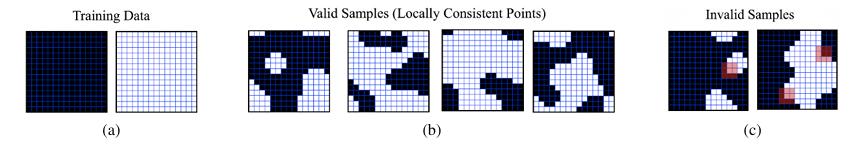
\includegraphics[width=0.9\textwidth]{../images/locally_consistent_point.png} % Change width and filename
\caption{
(a) A training set consisting of two images: one entirely black and one entirely white. 
(b) Creative samples produced by any local score-based model (LS or ELS) using a \(3 \times 3\) locality window with periodic boundary conditions. In this setup, local consistency requires that each generated pixel is either black or white, and that the majority color in every \(3 \times 3\) patch matches the color of its central pixel. 
(c) Samples are generated by numerically integrating the reverse diffusion process. If the integration step size is too large, local consistency can break down, resulting in invalid samples, as illustrated by the red-highlighted patches. In practice, for trained diffusion models, such local consistency typically holds only approximately~\cite{kamb2024analytictheorycreativityconvolutional}.
}   
\label{fig:local_consistency}
\end{figure}

\begin{theorem}
    Let \(x_T\) be a sample drawn from the distribution \(\pi_T\), and suppose this sample evolves according to the reverse process:
    \[
        \partial_t x_t = - \gamma_t \left( x_t + f^*(t,x_t) \right) \quad \text{with} \quad \gamma_t = -\frac{\partial_t \bar{\alpha}_t}{2 \bar \alpha_t}.
    \]
    Assuming the limits \( \lim\limits_{t \to 0} x_t \) and \( \lim\limits_{t \to 0} \partial_t x_t \) exist, the sample \( x_t \) converges to a locally consistent point.
\end{theorem}

\begin{proof}
    The assumption that \( \lim\limits_{t \to 0} \partial_t \bar \alpha_t \) and \( \lim\limits_{t \to 0} x_t \) exist implies that \( \gamma_t M_t(x_t) \) remains bounded as \( t \to 0 \).

    We have:
    \[
        \lim\limits_{t \to 0} v_{f^*,n}(t,x_t) (x) = \lim\limits_{t \to 0} - \frac{\partial_t \bar \alpha_t}{2\bar  \alpha_t (1 - \bar \alpha_t)} \sum_{x_0 \in P_{\Omega}} \left(x_t(n) - \sqrt{\bar{\alpha}_t} x_0[0]\right) W(x_0|x_t,n).
    \]

    With:
    \[
        W(x_0|x_t,n) = \frac{\mathcal{N}(\Sigma_n x_t | \sqrt{\bar{\alpha}_t} \varphi, (1 - \alpha_t)I)}
        {\sum\limits_{x_0' \in P_{\Omega}} \mathcal{N}(\Sigma_n x_t | \sqrt{\bar{\alpha}_t} \varphi', (1 - \alpha_t)I)}.
    \]

    Since 
    \[
        \lim\limits_{t \to 0} \frac{1}{1 - \bar \alpha_t} = +\infty 
        \quad \text{and} \quad 
        \frac{\partial_t \bar \alpha_t}{2 \bar \alpha_t} = \gamma_t \text{ exists and is continuous at } t=0,
    \]
    the sum on the right must tend to zero as \( t \to 0 \), that is:
    \[
        \lim\limits_{t \to 0} \sum_{x_0 \in P_{\Omega}} \left(x_t[n] - \sqrt{\bar{\alpha}_t} x_0[0]\right) W(x_0|x_t,n) = 0.
    \]

    We note that:
    \[
        \lim\limits_{t \to 0} W(x_0|x_t,n) =
        \begin{cases} 
        1, & \text{if } x_0 = x_0^* \coloneqq \arg \min_{x_0 \in P_{\Omega}} \|x_0 - \Sigma_n \tilde{x}\|^2. \\
        0, & \text{otherwise}.
        \end{cases}
    \]

    Thus, the limit of the sum reduces to:
    \[
        (x_0[n] - x_0^*[0]).
    \]

    The sum vanishing as \( t \to 0 \) implies:
    \[
        x_0[n] = x_0^*[0].
    \]
\end{proof}

\section{Analytical solutions for MMSE inverse problems}
In this section, we extend the analytical framework developed for MMSE denoising to the more general setting of inverse problems, where the observation model takes the form $y=Ax+b$. Unlike the denoising case where $A=I$, the presence of a general forward operator $A$ introduces new challenges related to the ill-posedness and instability of the inversion. Our goal is to characterize the MMSE estimator $\hat{x}(y)$ under architectural constraints such as locality and translation equivariance, as typically imposed by convolutional neural networks (CNNs). This project constitutes an ongoing research effort aimed to derive analytical formulas for the MMSE estimator under these constraints, with the mid-term objective of publishing the results. We target ICLR 2026 with a deadline for submission on September 2025. While the work is still in progress and some of the findings remain confidential, we already have preliminary results that offer valuable insights into the behavior of constrained neural estimators in inverse problem settings.

Note that this work is still ongoing, explaining the rather poor presentation below. I decided to focus on deriving new theoretical results rather than polishing the presentation. 

\subsection{Notations}
\begin{itemize}
    \item[]  $\x, \y, \beps$ are random vectors 
    \item[] Operator: $A: \R^N \to \R^M$, pseudo-inverse $A^+ : \R^M \to \R^N$
    \item[] Constrained set of functions: $\M = \{ \phi : \R^N \to \R^N: \dots \}$
\end{itemize}
Linear inverse problem:
\begin{equation*}
   \y = A \x + \beps 
\end{equation*}
The distribution of $\x$ is empirical, i.e.
\begin{equation}
    p_{\x}(u) =  \frac{1}{|\D|}\sum_{x\in\D} \delta(u-x)
\end{equation}
The distribution of $\y$ is given by
\begin{equation*}
    p_{\y}(v) = \frac{1}{|\D|}\sum_{x\in\D} \Normal{y,Ax,\sigma^2\Id_M}
\end{equation*}

\subsection{General}
\subsubsection{Problem}
We would like to solve
\begin{equation}\label{eq:general_problem}
    \min_{\phi \in \M} \E{\norm{\phi(\y) - \x}^2} \eqdef J(\phi)
\end{equation}
for some vector space $\M$. 
\subsubsection{Optimality condition}
$\phi^* \in \M$ is a minimizer of $J$ if $J(\phi^* + t \varphi) \geqslant J(\phi^*)$ for all $t \in \R$ and all $\varphi \in \M$. We have 
\begin{align*}
    J(\phi^* + t \varphi) &= \E{\norm{(\phi^* + t \varphi) (\y) - \x}^2} \\
    &= J(\phi^*) + t^2 \E{\norm{\varphi(\y)}^2} + 2t \E{\inner{\varphi(\y), \phi^*(\y) - \x}} 
\end{align*}
Therefore, the optimality condition is 
\begin{equation}\label{eq:optimality_condition}
    \E{\inner{\varphi(\y), \phi^*(\y) - \x}} = 0 \qquad \mbox{for all } \varphi \in \M
\end{equation}


% ############################################################################
% ----------------------------------------------------------------------------
% ----------------------------------------------------------------------------
% ------------------- INVERSE PROBLEMS ---------------------------------------
% ----------------------------------------------------------------------------
% ----------------------------------------------------------------------------
% ############################################################################


\subsubsection{Inverse problem: estimator with pseudo-inverse}
In this section, we are interested in finding the minimizer of the general problem \Cref{eq:general_problem} on a specific set of estimators:
\begin{equation*}
    \M = \left\{ \phi \circ A^+: \mbox{ for some } \phi: \R^N \to \R^N \right\}
\end{equation*}
and for the discrete data distribution. 
\\Firstly, the MMSE denoising without any constraint for inverse problem is given as follows.
\begin{proposition}[Unconstrained MMSE denoiser for inverse problem]
    The unconstrained MMSE denoiser is given by:
    \begin{equation}
        \phi^{*}(y) =  \frac{\sum_{x \in \D} x \Normal{y; A x, \sigma^2 \Id}}{\sum_{x \in \D} \Normal{y; A x, \sigma^2 \Id}} =   \frac{\sum_{x \in \D} x \exp \left( -\frac{\norm{A x - y}^2}{2 \sigma^2} \right) }{\sum_{x \in \D}  \exp \left( -\frac{\norm{A x - y}^2}{2 \sigma^2} \right) }
    \end{equation}
\end{proposition}
\begin{proof}
    We have
    \begin{align*}
        \E{\inner{\varphi(\y), \phi^*(\y) - \x}} &=\frac{1}{|\D|}\sum_{x\in\D}\int_{\R^M} \langle \varphi(y), \phi^*(y)-x\rangle \Normal{y,Ax,\sigma^2 \Id_M} dy\\
        &= \frac{1}{|\D|}\int_{\R^M} \left\langle \varphi(y), \phi^*(y) \sum_{x\in\D}\Normal{y,Ax,\sigma^2 \Id_M}-x \sum_{x\in\D}\Normal{y,Ax,\sigma^2 \Id_M}\right\rangle dy\\
        &=0
    \end{align*} 
\end{proof}

% \subsubsection{Translation equivariant estimator}
% We define 
% \begin{equation}
%     \M = \left\{ \phi \circ A^+, \phi: \R^N \to \R^N \mbox{ s.t } \phi(T_g x) = T_g \phi(x), \mbox{ for all } g \in G \right\},
% \end{equation}
% where $T_g$ is the translation operator.
\subsection{Local estimator}
We define 
\begin{equation}
    \M = \left\{\phi \circ A^+, \phi: \R^N \to \R^N \mbox{ s.t } \phi_n(x) = f_{\phi,n}(\Sigma_n x)\right\},
\end{equation}
where $\Sigma_n : \R^N \to \R^P$ ($P$ is the patch size) is the selection matrix and, $f_{\phi, n} : \R^P \to \R$ depends on $\phi$ and the pixel $n$.

\begin{proposition}[Local estimator for inverse problem]
    Suppose that $\det{\Sigma_n A^+ (\Sigma_n A^+)^T} = c \neq 0$ for all $n$ and $\dim(\Sigma_n \ker{A^+}) = M - P$.
    The local-MMSE is given by, for any patch $z \in \R^P$ with $M \geqslant P$: 
    \begin{equation*}
        f_{\phi^*, n}(z) = \frac{\sum_{x \in \D} x_n q(z, n, x)}{\sum_{x \in \D} q(z, n, x)}
    \end{equation*}
    where the weights are: 
    \begin{align*}
        q(z, n, x) = \Normal{S_{n}^{-1} U_{n}^T z; V_{n}^T A x, \sigma^2 \Id_{r_n}}
    \end{align*}
    where $\Sigma_n A^+ = U_n S_n V_n^T$ is the truncated SVD. 
\end{proposition}
\begin{proof}
 Inserting this estimator into the optimality \Cref{eq:optimality_condition}, for any $\varphi \in \M$:
\begin{align*}
    &\E{\inner{\varphi(A^+ \y), \phi^*(A^+  \y) - \x}}  \\
    &=  \frac{1}{|\D|} \int_{\R^M} \inner{\varphi(A^+  y), \phi^*(A^+  y) \sum_{x \in \D} \Normal{y; A x, \sigma^2 \Id_M} - \sum_{x \in \D} x \Normal{y; A x, \sigma^2 \Id_M}} dy \\
    &=  \frac{1}{|\D|} \sum_{n = 1}^{N} \int_{\R^M} \varphi_n (A^+  y) \left( \phi^*_n(A^+  y) \sum_{x \in \D} \Normal{y; A x, \sigma^2 \Id_M} - \sum_{x \in \D} x_n \Normal{y; A x, \sigma^2 \Id_M} \right) dy \\
    &=  \frac{1}{|\D|} \sum_{n = 1}^{N} \frac{1}{\det{S_n}} \int_{\R^M} f_{\varphi, n} (\Sigma_n A^+  y) \left( f_{\phi^*, n}(\Sigma_n A^+  y) \sum_{x \in \D} \Normal{y; A x, \sigma^2 \Id_N} - \sum_{x \in \D} x_n \Normal{y; A x, \sigma^2 \Id_N} \right) dy \\
    \\&= \frac{1}{|\D|} \sum_{n = 1}^{N} \frac{1}{\det{S_n}} \int_{\R^{r_n}} f_{\varphi, n} (U_{n}  z)  \Big(   f_{\phi^*, n}(U_{n}  z) \sum_{x \in \D} \Normal{S_{n}^{-1} z; V_{n}^T A x, \sigma^2 \Id_{r_n}} \\
    &\hspace{9cm} - \sum_{x \in \D} x_n \Normal{S_{n}^{-1} z; V_{n}^T A x, \sigma^2 \Id_{r_n}} \Big) dz
    \\&= 0
\end{align*}   
\end{proof}
\subsection{Local and translation equivariant estimator}
We define
\begin{equation}
    \M = \left\{\phi \circ A^+, \phi: \R^N \to \R^N \mbox{ s.t } \phi_n(x) = f_{\phi}(\Sigma_n x)\right\},
\end{equation}
a set of local and translation equivariant functions. Unlike the local denoiser, the mapping $f_{\phi}$ is now independent of the pixel location $n$, meaning the function behaves identically across all positions.

Translation property: the translation is defined as $T_g : (x_1, \dots, x_N) \in \R^N \mapsto (x_{1 - g}, \dots, x_{N - g}) \in \R^N$, then we have: $\Sigma_n T_g x = \Sigma_{n - g} x$ for all $g$ and all $x \in \R^N$ (translate + crop is the same as crop the translated location). Therefore, the functions $\phi$ are translation equivariant in the sense that $\phi(T_g x) = T_g \phi(x)$.
\begin{proposition}[Local estimator and translation equivariant for inverse problem]
    Suppose that $\det{\Sigma_n A^+ (\Sigma_n A^+)^T} = c \neq 0$ for all $n$.
    The local and translation-equivariant MMSE is given by, for any patch $z \in \R^P$ with $M \geqslant P$: 
    \begin{equation*}
        f_{\phi^*}(z) = \frac{\sum_{x \in \D} \sum_{n = 1}^{N} x_n q(z, n, x)}{\sum_{x \in \D} \sum_{n = 1}^{N} q(z, n, x)}
    \end{equation*}
    where the weights are: 
    \begin{align*}
        q(z, n, x) &= \int_{v_n^{-1}(z)} \Normal{w; A x, \sigma^2 \Id} d \H^{M - P}(w) 
        \\&= \frac{1}{(2\pi \sigma^2)^{P/2}} \exp \left( -\frac{\norm{(\Id_M - V_n V_n^T)A x - (\Sigma_n A^+)^+ z}^2}{2\sigma^2} \right)
    \end{align*}

    \begin{align*}
        q(z, n, x) &= \frac{1}{(2\pi \sigma^2)^{P/2}} \exp \left( -\frac{\norm{(\Id_M - V_n V_n^T)A x - (\Sigma_n A^+)^+ z}^2}{2\sigma^2} \right)
    \end{align*}
    with $v_n: w \in \R^M \mapsto \Sigma_n A^+ w \in \R^P$ and $V_n$ is an orthogonal basis of $\ker{\Sigma_n A^+}$.
\end{proposition}
\begin{proof}
Inserting this estimator into the optimality \Cref{eq:optimality_condition}, for any $\varphi \in \M$:
\begin{align*}
    &\E{\inner{\varphi(A^+ \y), \phi^*(A^+  \y) - \x}}  \\
    &=  \frac{1}{|\D|} \int_{\R^M} \inner{\varphi(A^+  y), \phi^*(A^+  y) \sum_{x \in \D} \Normal{y; A x, \sigma^2 \Id_N} - \sum_{x \in \D} x \Normal{y; A x, \sigma^2 \Id_N}} dy \\
    &=  \frac{1}{|\D|} \sum_{n = 1}^{N} \int_{\R^M} \varphi_n (A^+  y) \left( \phi^*_n(A^+  y) \sum_{x \in \D} \Normal{y; A x, \sigma^2 \Id_N} - \sum_{x \in \D} x_n \Normal{y; x, \sigma^2 \Id_N} \right) dy \\
    &=  \frac{1}{|\D|} \sum_{n = 1}^{N} \int_{\R^M} f_{\varphi} (\Sigma_n A^+  y) \left( f_{\phi^*}(\Sigma_n A^+  y) \sum_{x \in \D} \Normal{y; A x, \sigma^2 \Id_N} - \sum_{x \in \D} x_n \Normal{y; A x, \sigma^2 \Id_N} \right) dy \\
    &=  \frac{1}{|\D|} \sum_{n = 1}^{N} \int_{\R^P} \int_{v_n^{-1}(z)} f_{\varphi} (\Sigma_n A^+ w) \left( f_{\phi^*}(\Sigma_n A^+ w) \sum_{x \in \D} \Normal{w; A x, \sigma^2 \Id_N} \right. 
    \\& \left. \hspace{7cm} -\sum_{x \in \D} x_n \Normal{w; A x, \sigma^2 \Id_N} \right) d\H^{M - P}(w) dz \\
    &=  \frac{1}{|\D|}  \int_{\R^P} f_{\varphi}(z) \left(  f_{\phi^*}(z) \sum_{x \in \D} \sum_{n = 1}^{N} \int_{v_n^{-1}(z)} \Normal{w; A x, \sigma^2 \Id_N} d\H^{M-P}(z) \right. 
    \\& \left. \hspace{7cm} - \sum_{x \in \D} \sum_{n = 1}^{N} x_n \int_{v_n^{-1}(z)} \Normal{w; A x, \sigma^2 \Id_N} d\H^{M-P}(z)\right) dz \\
    % &=  \frac{1}{|\D|} \int_{\R^P} f_{\varphi}(z) \left(  f_{\phi^*}(z) \sum_{x \in \D} \sum_{n = 1}^{N} q(z, n, x)  -  \sum_{x \in \D} \sum_{n = 1}^{N} x_n q(z, n, x) \right) dz
    % \\&= \frac{1}{|\D|} \sum_{n = 1}^{N} \frac{1}{\det{S_n}} \int_{\R^{r_n}} f_{\varphi} (U_n z) \left( f_{\phi^*}(U_n z) \sum_{x \in \D} \Normal{S_n^{-1} z; V_n^T A x, \sigma^2 \Id_{r_n}} - \sum_{x \in \D} x_n \Normal{S_n^{-1} z; V_n^T A x, \sigma^2 \Id_{r_n}} \right) dy
    % \\&=\frac{1}{|\D|} \int_{\R^{P}}  f_{\varphi} (v)  \left( f_{\phi^*}(v)  \sum_{x \in \D}  \sum_{n = 1}^N \sum_{z \in U_n^{-}(v)} \frac{\Normal{S_n^{-1} z; V_n^T A x, \sigma^2 \Id_{r_n}}}{\det{S_n}}  - \sum_{x \in \D}  \sum_{n = 1}^N  \sum_{z \in U_n^{-}(v)} \frac{x_n \Normal{S_n^{-1} z; V_n^T A x, \sigma^2 \Id_{r_n}}}{\det{S_n}} \right) d \H^{r_n}(v)
    \\&= 0 
\end{align*}
\end{proof}

% \subsubsection{Group equivariant estimator}
% Consider a general group of transformations $G$. 
% We define 
% \begin{equation}
%     \M = \left\{ \phi \circ A^+, \phi : \R^N \to \R^N \mbox{ s.t } \phi(T_g x) = T_g \phi(x) \right\},
% \end{equation}
% the set of group equivariant constraint. \textbf{The function $\phi$ are group equivariant but the composition $\phi \circ A^+$ might be not}. 

% \subsubsection{Local and group equivariant estimator}

% \section{Inverse problem: estimator with generalized group of transformations}
% \subsubsection{Preliminaries on equivariance}
% The below definitions are taken from \cite{Celledoni_2021_equivariant_neural_networks}. 
% \begin{definition}[Group] A \emph{group}, to be denoted $G$, is a set equipped with an associative operator $\cdot : G \times G \to G$, which satisfies the following conditions:
%     \begin{enumerate}
%         \item[] If $g_1, g_2 \in G$ then $g_2 \cdot g_1 \in G$
%         \item[] If $g_1, g_2, g_3 \in G$ then $(g_1 \cdot g_2) \cdot g_3 = g_1 \cdot (g_2 \cdot g_3)$
%         \item[] There exists $e \in G$ such that $e \cdot g = g \cdot e = g$ for all $g \in G$.
%         \item[] If $g \in G$ there exists $g^{-1} \in G$ such that $g^{-1} \cdot g = g \cdot g^{-1} = e$.
%     \end{enumerate}    
% \end{definition}
% \begin{definition}[Group action]
%     Given a group $G$ and a set $\X \subset \R^N$, we say that $G$ acts on $\X$ if there exists a function $T: G \times \X \to \X$ (we denote by $T_g(x)$ for $g \in G$ and $x \in \X$) that satisfies:
%     \begin{equation*}
%         T_{g_1} \circ T_{g_2} = T_{g_1 \cdot g_2} \qquad \mbox{and} \qquad T_{e} = \mathrm{id}
%     \end{equation*} 
% \end{definition}
% \begin{example}
%     The Euclidean group $E(N)$ is the group generated by translations, rotations and reflections in $\R^N$. For which the group action can be represented by a translation $T_g$, an orthogonal matrix $R_g$ that rotates or reflects coordinates. 
% \end{example}

% \begin{definition}[Equivariance estimator]
% Given a general group $G$. A function $\phi: \Y \to \X$ and group actions $\Tx, \Ty$ of $G$ on $\X, \Y$, $\phi$ is called \emph{equivariant} if it satisfies
% \begin{equation*}
%     \phi(\Ty_g(y)) = \Tx_g \phi(y) \qquad \mbox{for all } x \in \X \mbox{ and for all } g \in G.
% \end{equation*}
% \end{definition}
% \textbf{Question}: how to define the group actions $\Tx$ and $\Ty$?
% Given a linear operator $A: \X \to \Y$ and a group action $\Tx$ of $G$ acting on $\X$, we can for example define the following group action on $\Y$ \cite{beckmann2024equivariantneuralnetworksindirect}:
% \begin{align*}
%     \Ty_g : \Y & \to \Im{A} \subset \Y \\ 
%                y      & \mapsto T_g^{\Y}(y) = A T_g^{\X}(A^+y) 
% \end{align*}
% \begin{proposition}[From \cite{Celledoni_2021_equivariant_neural_networks}]
%     A linear function $\phi: \Y \to \X$ is equivariant if and only if it is defined by a convolution.
% \end{proposition}

% \begin{proposition}
%     If the group $G$ is finite, the following properties hold true:
%     \begin{enumerate}
%         \item[] \textbf{Invariance}: for any function $\phi: \X \to \R$, the function $\bar{\phi}(y) = \sum_{g} \phi(\Tx_g y)$ is in variant. (And similarly for function defined in $\Y$).  
%         \item[] \textbf{Equivariance}: for any function $\phi: \Y \to \X$, the function $\bar{\phi}(y) = \sum_{g} \left( \Tx_g \right)^{-1} \phi (\Ty_g y)$ is equivariant. This is called \textbf{Reynolds averaging}.
%     \end{enumerate} 
% \end{proposition}

% \subsubsection{Group equivariant estimator}
% Consider a general group $G$ with its actions $\Tx$ and $\Ty$ on $\X$ and $\Y$, respectively (where $\X = \R^N$ and $\Y = \R^M$). 
% We define 
% \begin{equation}
%     \mathcal{M} = \left\{ \phi: \Y \to \X \mbox{ s.t } \phi(\Ty_g y) = \Tx_g \phi(y) \right\}
% \end{equation}
% the set of group equivariant estimators.
% \begin{proposition}[Group equivariant estimator]
%     \textbf{If $\Tx, \Ty$ are orthogonal isometry}, the group equivariant estimator is given by 
%     \begin{equation}
%         \phi^{*}(y) = \frac{\sum_{x \in \D} \sum_{g \in G} \Tx_g x \Normal{y; \Ty_g A x, \sigma^2 \Id}}{ \sum_{x \in \D} \sum_{g \in G} \Normal{y; \Ty_g A x, \sigma^2 \Id}}
%     \end{equation}
% \end{proposition}
% Inserting this estimator into the optimality \Cref{eq:optimality_condition}, for any $\varphi \in \M$:
% \begin{align*}
%     &\E{\inner{\varphi(\y), \phi^*(\y) - \x}}  \\
%     &=  \frac{1}{|\D|} \int_{\R^M} \inner{\varphi(y), \phi^*(y) \sum_{x \in \D} \Normal{y; A x, \sigma^2 \Id_N} - \sum_{x \in \D} x \Normal{y; A x, \sigma^2 \Id_N}} dy
%     \\&= \frac{1}{|\D| |G|} \int_{\R^M} \inner{\varphi(y), \phi^*(y) \sum_{x \in \D, g \in G} \Normal{\Ty_g y; \Ty_g A x, \sigma^2 \Id_N} - \sum_{x \in \D, g \in G} x \Normal{\Ty_g y; \Ty_g A x, \sigma^2 \Id_N}} dy
%     \\&= \frac{1}{|\D| |G|} \sum_{g \in G} \int_{\R^M} \inner{ (\Tx_g)^{-1} \varphi(\Ty_g y), (\Tx_g)^{-1} \phi^*(\Ty_g y) \sum_{x \in \D} \Normal{\Ty_g y; \Ty_g A x, \sigma^2 \Id_N} - \sum_{x \in \D} x \Normal{\Ty_g y; \Ty_g A x, \sigma^2 \Id_N}} dy
%     \\&= \frac{1}{|\D| |G|} \sum_{g \in G} \int_{\R^M} \inner{(\Tx_g)^{-1} \varphi(y), (\Tx_g)^{-1} \phi^*(y) \sum_{x \in \D} \Normal{y; \Ty_g A x, \sigma^2 \Id_N} - \sum_{x \in \D} x \Normal{y; \Ty_g A x, \sigma^2 \Id_N}} dy
%     \\&= \frac{1}{|\D| |G|} \sum_{g \in G} \int_{\R^M} \inner{(\Tx_g)^{-T}(\Tx_g)^{-1} \varphi(y),  \phi^*(y) \sum_{x \in \D} \Normal{y; \Ty_g A x, \sigma^2 \Id_N} - \sum_{x \in \D} \Tx_g x \Normal{y; \Ty_g A x, \sigma^2 \Id_N}} dy
%     \\&= \frac{1}{|\D| |G|} \int_{\R^M} \inner{\varphi(y),  \phi^*(y) \sum_{x \in \D} \sum_{g \in G} \Normal{y; \Ty_g A x, \sigma^2 \Id_N} - \sum_{x \in \D} \sum_{g \in G} \Tx_g x \Normal{y; \Ty_g A x, \sigma^2 \Id_N}} dy
%     \\&= 0
% \end{align*}

% {
%     \color{blue}
%     \textbf{Note:} this requires the transformations in the image domain $\Tx$ and in the measurement domain $\Ty$ are \textbf{linear orthogonal transformations}. This should be defined properly for each operator $A$. 
% }

\section{Conclusion}
The primary aim of this work was to understand the behavior of CNNs, in inverse problems by analyzing MMSE estimator under architectural constraints such as locality and translation equivariance. By extending the analytical framework introduced by Ganguli et al. (2024) \cite{kamb2024analytictheorycreativityconvolutional} in the denoising setting, we sought to uncover how these structural priors alone influence the learned estimators, without requiring full access to training dynamics or data distributions.

Our main result demonstrates that, in the context of linear inverse problems $y=Ax+b$, imposing local and translation equivariance on the estimator yields non trivial analytical expression. 
Analyzing this expression will provide us some insights on what type of image can be recovered when solving inverse problems with neural networks. 
Certifying and understanding the solution of neural networks in the context of inverse problems is a critical issue. Imagine for instance a solver for a magnetic imaging reconstruction. 
Diagnosing a brain tumor while it is not there (or vice versa) could have dramatic consequences. 

Our findings align with and build upon recent theoretical studies that investigate the inductive biases of neural architectures, but differ by providing closed-form analytical characterizations rather than empirical or asymptotic analyses.

Nonetheless, this analysis still requires some work. First, a validation on realistic datasets and comparison with trained networks remains to be done. Second, a deeper analysis of the analytical formulas, with some simple examples will help to get insight on these otherwise hard to read equations. I hope that my summer internship will enable me addressing these issues and to publish a nice paper!

\section{Appendix}

\subsection{Proof of \Cref{prop:fokker} \label{sec:proof_focker}}

% \begin{proof}
% Let's start with a reminder of Itô's formula. 
% \begin{theorem}[Formule d'Itô \cite{Oksendal2003}]
% Soit \( X(t) \) un processus d’Itô de dimension \( n \) vérifiant  
% \[
% dX(t) = u(t, X(t)) dt + v(t, X(t)) dB(t),
% \]
% où :
% \begin{itemize}
%     \item[] \( X(t) \in \mathbb{R}^n \) est le processus d’état,
%     \item[] \( u(t, X(t)) \in \mathbb{R}^n \) est le terme de dérive,
%     \item[] \( v(t, X(t)) \in \mathbb{R}^{n \times m} \) est la matrice de diffusion,
%     \item[] \( B(t) \in \mathbb{R}^m \) est un mouvement brownien standard de dimension \( m \).
% \end{itemize}

% Soit \( g: [0, \infty) \times \mathbb{R}^n \to \mathbb{R}^p \) une fonction deux fois continûment différentiable.  
% On définit le processus transformé :
% \[
% Y(t) = g(t, X(t)),
% \]
% où \( Y(t) \in \mathbb{R}^p \).  
% Alors, \( Y(t) \) satisfait l’équation d’Itô :
% \[
% dY_k = \frac{\partial g_k}{\partial t} dt 
% + \sum\limits_{i=1}^{n} \frac{\partial g_k}{\partial x_i} u_i dt 
% + \sum\limits_{i=1}^{n} \sum\limits_{j=1}^{m} \frac{\partial g_k}{\partial x_i} v_{ij} dB_j
% + \frac{1}{2} \sum\limits_{i,j=1}^{n} \sum\limits_{r=1}^{m} v_{ir} v_{jr} \frac{\partial^2 g_k}{\partial x_i \partial x_j} dt.
% \]
% \end{theorem}
% \vspace{3em}



% Soit une fonction test $F: \mathbb{R}^N \rightarrow \mathbb{R}$, de classe $C^{\infty}$, à support compact. En utilisant la formule d'Ito, on obtient
% %     \[dF(x_t) = \sum\limits_{i=1}^N \frac{\partial F(x_t)}{\partial x_i} dx_t^i + \frac{1}{2} \sum\limits_{i=1}^N \sum\limits_{j=1}^N \frac{\partial^2 F(x_t)}{\partial x_i^2}d\langle x^i,x^j\rangle_t\]
% % En utilisant l'équation \Cref{eq:SDE} et en notant que 
% %  on obtient:
% \begin{align*}
%     dF(x_t) &= \sum\limits_{i=1}^N \frac{\partial F(x_t)}{\partial x_i} (f^i_t(x_t)dt + \mathcal{G}_tdW^i_t) + \frac{1}{2} \sum\limits_{i=1}^N  \frac{\partial^2 F(x_t)}{\partial x_i^2} \mathcal{G}_t^2 dt \\
%     &= \left(\sum\limits_{i=1}^N \frac{\partial F(x_t)}{\partial x_i} f^i_t(x_t) + \frac{1}{2} \sum\limits_{i=1}^N  \frac{\partial^2 F(x_t)}{\partial x_i^2} \mathcal{G}_t^2\right)dt + \sum\limits_{i=1}^N \frac{\partial F(x_t)}{\partial x_i}  \mathcal{G}_t^2dW^i_t
% \end{align*}

% The $dW_t^i$ term disappears when taking the expectation (because $\E{dW_t^i} = 0$ ), so :
% \[\E{dF(x_t)} = \E{\left(\sum\limits_{i=1}^N \frac{\partial F(x_t)}{\partial x_i} f^i_t(x_t) + \frac{1}{2} \sum\limits_{i=1}^N \frac{\partial^2 F(x_t)}{\partial x_i^2} \mathcal{G}_t^2\right)dt}\]

% Ou encore, en utilisant la linéarité de l'opérateur espérance, on peut sortir la dérivée, l'équation ci-dessus s'écrit :
% \[ d\E{F(x_t)} = \E{\sum\limits_{i=1}^N \frac{\partial F(x_t)}{\partial x_i} f^i_t(x_t) + \frac{1}{2} \sum\limits_{i=1}^N \frac{\partial^2 F(x_t)}{\partial x_i^2} \mathcal{G}_t^2}dt\]

% Ainsi,
% \begin{align}
%     \frac{d\E{F(x_t)}}{dt} &= \E{\sum\limits_{i=1}^N \frac{\partial F(x_t)}{\partial x_i} f^i_t(x_t) + \frac{1}{2} \sum\limits_{i=1}^N  \frac{\partial^2 F(x_t)}{\partial x_i^2}\mathcal{G}_t^2} \nonumber \\
%     &=\E{\sum\limits_{i=1}^N \frac{\partial F(x_t)}{\partial x_i} f^i_t(x_t)} + \E{\frac{1}{2} \sum\limits_{i=1}^N  \frac{\partial^2 F(x_t)}{\partial x_i^2} \mathcal{G}_t^2} \nonumber\\
%     &=\E{ \nabla\ F(x_t) \cdot f_t(x_t)} + \frac{1}{2}\E{\nabla^2 F(x_t) \mathcal{G}_t^2} \label{eq:EsperanceEgality}
% \end{align}

% $F$ est continue, donc mesurable, supposons que $x \rightarrow \frac{\partial\pi_t(x)}{\partial t}$ existe, $x \rightarrow F(x)\frac{\partial\pi_t(x)}{\partial t}$ est intégrable en $\R^N$ car F est à support compact. D'après la règle de Leibniz, le premier terme à droite s'écrit :
% \[\frac{d\mathbb{E}[F(x_t)]}{dt} = \frac{d (\int_{\mathbb{R^N}} F(x) \pi_t(x) dx)} {dt} = \int_{\mathbb{R^N}}F(x)\frac{\partial\pi_t(x)}{\partial t} dx\]
% \vspace{2em}

% Nous allons rappeler la première identité de Green (Green's first identity) qui est fort utile dans la suite.

% \begin{theorem}[Première identité de Green]
% Soit $\Omega \subset \R^n$, on se donne une fonction $u : \Omega \rightarrow \R$, $u \in C^2$ et une autre fonction $v : \Omega \rightarrow \R$, $v \in C^1$, alors :
% \begin{equation}\label{eq:GreenId}
% \int_\Omega (v(x)\nabla^2 u(x) + \nabla u(x) \cdot \nabla v(x)) dx = \int_{\partial\Omega} v \nabla u \cdot n dS
% \end{equation}
% Avec n le vecteur normal unitaire à la frontière $\partial\Omega$ et $dS$ la mesure de frontière sur $\partial\Omega$.
% \end{theorem}
% \vspace{3em}

% Supposons qu'il existe une fonction $v_t$ telle que $\nabla_{x} v_t = f_t \pi_t$.

% On utilise la première identité de Green sur le premier terme à gauche en remarquant que l'intégrale sur le bord s'annule car F est à support compact, on obtient :
% \begin{align*}
%     \E{\nabla\ F(x_t)\cdot f_t(x_t)}  &=\int_{\mathbb{R^N}} \nabla\ F(x)\cdot \big(f_t(x) \pi_t(x) \bigr)dx \\
%     &= - \int_{\mathbb{R}^N}F(x) (\nabla \cdot f_t(x)\pi_t(x))dx
% \end{align*}

% De la même manière, en appliquant l'intégration par parties deux fois sur le deuxième terme à droite, on obtient :
% \begin{align*}
%     \E{\nabla^2 F(x_t) \mathcal{G}_t^2} &= \int_{\mathbb{R}^N } \nabla^2 F(x) \mathcal{G}_t^2 \pi_t(x)dx\\
%     &= -\int_{\R^N}\nabla F(x) \cdot\nabla(\mathcal{G}_t^2\pi_t(x)) dx\\
%     &= \int_{\mathbb{R}^N } F(x) \nabla^2(\mathcal{G}_t^2 \pi_t(x)) dx
% \end{align*}

% Injectons les résultats précédents dans l'équation \Cref{eq:EsperanceEgality} :
% \[\int_{\mathbb{R^N}}F(x)\frac{\partial\pi_t(x)}{\partial t} dx = - \int_{\mathbb{R}^N}F(x) (\nabla \cdot f_t(x)\pi_t(x))dx + \frac{1}{2}\int_{\mathbb{R}^N } F(x) \nabla^2(\mathcal{G}_t^2 \pi_t(x)) dx\]

% Cette relation est vraie pour toute fonction de test $F \in C_c^{\infty}$ (i.e. ensemble des fonctions infiniment dérivables à support compact), la théorie des distributions nous dit : 
% \[\frac{\partial\pi_t(x)}{\partial t} = -\nabla \cdot (f_t(x)\pi_t(x)) + \frac{1}{2}\nabla^2(\mathcal{G}_t^2 \pi_t(x)) \quad \] 
% \end{proof}

Let us begin with a reminder of Itô's formula.
\begin{theorem}[Itô's Formula \cite{Oksendal2003}]
Let \( X(t) \) be an Itô process in \( \mathbb{R}^n \) satisfying  
\[
dX(t) = u(t, X(t)) dt + v(t, X(t)) dB(t),
\]
where:
\begin{itemize}
    \item[] \( X(t) \in \mathbb{R}^n \) is the state process,
    \item[] \( u(t, X(t)) \in \mathbb{R}^n \) is the drift term,
    \item[] \( v(t, X(t)) \in \mathbb{R}^{n \times m} \) is the diffusion matrix,
    \item[] \( B(t) \in \mathbb{R}^m \) is an \( m \)-dimensional standard Brownian motion.
\end{itemize}
Let \( g: [0, \infty) \times \mathbb{R}^n \to \mathbb{R}^p \) be a function that is twice continuously differentiable.  
we define the transformed process:
\[
Y(t) = g(t, X(t)),
\]
where \( Y(t) \in \mathbb{R}^p \).  
Then \( Y(t) \) satisfies the Itô equation:
\[
dY_k = \frac{\partial g_k}{\partial t} dt 
+ \sum\limits_{i=1}^{n} \frac{\partial g_k}{\partial x_i} u_i dt 
+ \sum\limits_{i=1}^{n} \sum\limits_{j=1}^{m} \frac{\partial g_k}{\partial x_i} v_{ij} dB_j
+ \frac{1}{2} \sum\limits_{i,j=1}^{n} \sum\limits_{r=1}^{m} v_{ir} v_{jr} \frac{\partial^2 g_k}{\partial x_i \partial x_j} dt.
\]
\end{theorem}
Let \( F: \mathbb{R}^N \rightarrow \mathbb{R} \) be a smooth test function with compact support. Using Itô’s formula, we obtain
\begin{align*}
    dF(x_t) &= \sum\limits_{i=1}^N \frac{\partial F(x_t)}{\partial x_i} (f^i_t(x_t)dt + \mathcal{G}_t dW^i_t) + \frac{1}{2} \sum\limits_{i=1}^N  \frac{\partial^2 F(x_t)}{\partial x_i^2} \mathcal{G}_t^2 dt \\
    &= \left(\sum\limits_{i=1}^N \frac{\partial F(x_t)}{\partial x_i} f^i_t(x_t) + \frac{1}{2} \sum\limits_{i=1}^N  \frac{\partial^2 F(x_t)}{\partial x_i^2} \mathcal{G}_t^2\right)dt + \sum\limits_{i=1}^N \frac{\partial F(x_t)}{\partial x_i}  \mathcal{G}_t dW^i_t
\end{align*}
The \( dW_t^i \) term vanishes when taking the expectation (since \( \mathbb{E}[dW_t^i] = 0 \)), so:
\[
\mathbb{E}[dF(x_t)] = \mathbb{E}\left[\left(\sum\limits_{i=1}^N \frac{\partial F(x_t)}{\partial x_i} f^i_t(x_t) + \frac{1}{2} \sum\limits_{i=1}^N \frac{\partial^2 F(x_t)}{\partial x_i^2} \mathcal{G}_t^2\right)dt\right]
\]
Or, using the linearity of expectation to factor out the derivative:
\[
d\mathbb{E}[F(x_t)] = \mathbb{E}\left[\sum\limits_{i=1}^N \frac{\partial F(x_t)}{\partial x_i} f^i_t(x_t) + \frac{1}{2} \sum\limits_{i=1}^N \frac{\partial^2 F(x_t)}{\partial x_i^2} \mathcal{G}_t^2\right]dt
\]
Thus,
\begin{align}
    \frac{d\mathbb{E}[F(x_t)]}{dt} &= \mathbb{E}\left[\sum\limits_{i=1}^N \frac{\partial F(x_t)}{\partial x_i} f^i_t(x_t) + \frac{1}{2} \sum\limits_{i=1}^N  \frac{\partial^2 F(x_t)}{\partial x_i^2}\mathcal{G}_t^2\right] \nonumber \\
    &= \mathbb{E}\left[\sum\limits_{i=1}^N \frac{\partial F(x_t)}{\partial x_i} f^i_t(x_t)\right] + \mathbb{E}\left[\frac{1}{2} \sum\limits_{i=1}^N  \frac{\partial^2 F(x_t)}{\partial x_i^2} \mathcal{G}_t^2\right] \nonumber\\
    &= \mathbb{E}[ \nabla F(x_t) \cdot f_t(x_t)] + \frac{1}{2}\mathbb{E}[\nabla^2 F(x_t) \mathcal{G}_t^2] \label{eq:EsperanceEgality}
\end{align}
Since \( F \) is continuous, it is measurable. Suppose that \( x \mapsto \frac{\partial\pi_t(x)}{\partial t} \) exists. Then \( x \mapsto F(x)\frac{\partial\pi_t(x)}{\partial t} \) is integrable on \( \mathbb{R}^N \) because \( F \) has compact support. By Leibniz's rule, the first term on the right becomes:
\[
\frac{d\mathbb{E}[F(x_t)]}{dt} = \frac{d}{dt} \left(\int_{\mathbb{R}^N} F(x) \pi_t(x) dx\right) = \int_{\mathbb{R}^N}F(x)\frac{\partial\pi_t(x)}{\partial t} dx
\]
\vspace{2em}
We now recall Green’s first identity
\begin{theorem}[Green’s First Identity]
Let \( \Omega \subset \mathbb{R}^n \), and suppose \( u : \Omega \rightarrow \mathbb{R} \), \( u \in C^2 \), and \( v : \Omega \rightarrow \mathbb{R} \), \( v \in C^1 \), then:
\begin{equation}\label{eq:GreenId}
\int_\Omega (v(x)\nabla^2 u(x) + \nabla u(x) \cdot \nabla v(x)) dx = \int_{\partial\Omega} v \nabla u \cdot n dS
\end{equation}
where \( n \) is the outward unit normal vector on the boundary \( \partial\Omega \), and \( dS \) is the surface measure on \( \partial\Omega \).
\end{theorem}
Suppose a function \( v_t \) exists such that \( \nabla_x v_t = f_t \pi_t \).
Using Green’s first identity on the first term on the left and noting that the boundary integral vanishes because \( F \) has compact support, we obtain:
\begin{align*}
    \mathbb{E}[\nabla F(x_t)\cdot f_t(x_t)] &=\int_{\mathbb{R}^N} \nabla F(x)\cdot (f_t(x) \pi_t(x)) dx \\
    &= - \int_{\mathbb{R}^N}F(x) (\nabla \cdot (f_t(x)\pi_t(x))) dx
\end{align*}
Similarly, applying integration by parts twice on the second term on the right yields:
\begin{align*}
    \mathbb{E}[\nabla^2 F(x_t) \mathcal{G}_t^2] &= \int_{\mathbb{R}^N } \nabla^2 F(x) \mathcal{G}_t^2 \pi_t(x) dx \\
    &= -\int_{\mathbb{R}^N} \nabla F(x) \cdot \nabla(\mathcal{G}_t^2\pi_t(x)) dx \\
    &= \int_{\mathbb{R}^N} F(x) \nabla^2(\mathcal{G}_t^2 \pi_t(x)) dx
\end{align*}
Substituting the results into equation \Cref{eq:EsperanceEgality}:
\[
\int_{\mathbb{R}^N}F(x)\frac{\partial\pi_t(x)}{\partial t} dx = - \int_{\mathbb{R}^N}F(x) (\nabla \cdot (f_t(x)\pi_t(x))) dx + \frac{1}{2}\int_{\mathbb{R}^N } F(x) \nabla^2(\mathcal{G}_t^2 \pi_t(x)) dx
\]
This relation holds for all test functions \( F \in C_c^{\infty} \) (i.e., smooth functions with compact support), so by distribution theory:
\[
\frac{\partial\pi_t(x)}{\partial t} = -\nabla \cdot (f_t(x)\pi_t(x)) + \frac{1}{2}\nabla^2(\mathcal{G}_t^2 \pi_t(x))
\]


\subsection{Proof of \Cref{prop:solution_processus_direct}} \label{sec:proof_solution_processus_direct}
According to equation \Cref{eq:OU}:
\begin{equation*}
dx_t^i = -\gamma_t x_t^i dt + \sqrt{2\gamma_t} dW_t^i, \quad \forall i=1,2,\dots,N
\end{equation*}
Let $\mu_t = \exp\left(\int_0^t \gamma_s ds\right)$, $\forall t \geq 0$.
Define a stochastic process $Y_t$ by $Y_t \coloneqq f(t, x_t^i) = \mu_t x_t^i$.
Using Itô's formula, we obtain:
\begin{equation*}
dY_t = \frac{\partial f(t, x_t^i)}{\partial t} dt + \frac{\partial f(t, x_t^i)}{\partial x} dx_t + \frac{1}{2} \frac{\partial^2 f(t, x_t^i)}{\partial x^2} d\langle x, x \rangle_t
\end{equation*}
In particular:
\begin{itemize}
    \item[] $\frac{\partial f(t, x_t^i)}{\partial t} = \gamma_t \mu_t x_t^i$
    \item[] $\frac{\partial f(t, x_t^i)}{\partial x} = \mu_t$
    \item[] $\frac{\partial^2 f(t, x_t^i)}{\partial x^2} = 0$
\end{itemize}
Thus,
\begin{align*}
dY_t &= \gamma_t \mu_t x_t^i dt + \mu_t dx_t^i \\
&= \gamma_t \mu_t x_t^i dt + \mu_t \left(-\gamma_t x_t^i dt + \sqrt{2\gamma_t} dW_t^i\right) \\
&= \mu_t \sqrt{2\gamma_t} dW_t^i
\end{align*}
Integrating both sides, we get:
\begin{equation*}
Y_t = Y_0 + \int_0^t \mu_s \sqrt{2\gamma_s} dW_s^i
\end{equation*}
Substituting $Y_t = \mu_t x_t^i$ and dividing both sides by $\mu_t$ to isolate $x_t^i$, we obtain:
\begin{align*}
x_t^i &= \frac{1}{\mu_t} x_0^i + \frac{1}{\mu_t} \int_0^t \mu_s \sqrt{2\gamma_s} dW_s^i \\
&= \sqrt{\bar{\alpha}_t} x_0^i + \frac{1}{\mu_t} \int_0^t \mu_s \sqrt{2\gamma_s} dW_s^i
\end{align*}
Let $Z_t = \int_0^t \mu_s \sqrt{2\gamma_s} dW_s^i$. Notice that $Z_t$ is an Itô integral with respect to a Brownian motion. We can express this integral as:
\begin{equation*}
Z_t = \int_0^t \mu_s \sqrt{2\gamma_s} dW_s^i = \lim_{h \to 0} \sum_{j=1}^n \mu_{t_j} \sqrt{2\gamma_{t_j}} (W_{t_j}^i - W_{t_{j-1}}^i)
\end{equation*}
where $t_0 = 0 < t_1 < \dots < t_{n-1} < t_n = t$ is a partition of the interval $[0, t]$, and $h \coloneqq \max_{j=1,2,\dots,n} |t_j - t_{j-1}|$.
\\Since the increments of a Brownian motion are centered, independent Gaussian random variables, $Z_t$ is a centered Gaussian random variable with variance $\int_0^t (\mu_s \sqrt{2\gamma_s})^2 ds$. Let us compute this variance:
\begin{align*}
\int_0^t (\mu_s \sqrt{2\gamma_s})^2 ds &= \int_0^t \exp\left(2 \int_0^s \gamma_x dx\right) 2 \gamma_s ds \\
&= \int_0^t \exp\left(2 \int_0^s \gamma_x dx\right) d\left(2 \int_0^s \gamma_x dx\right) \\
&= \exp\left(2 \int_0^t \gamma_x dx\right) - 1
\end{align*}
Thus, $Z_t$ is a Gaussian random variable such that:
\begin{equation*}
Z_t \sim \mathcal{N}\left(0, \exp\left(2 \int_0^t \gamma_x dx\right) - 1\right)
\end{equation*}
Consequently,
\begin{equation*}
\frac{1}{\mu_t} Z_t \sim \mathcal{N}\left(0, 1 - \exp\left(-2 \int_0^t \gamma_x dx\right)\right)
\end{equation*}
Hence:
\begin{equation*}
\frac{1}{\mu_t} Z_t \sim \mathcal{N}\left(0, 1 - \bar{\alpha}_t\right)
\end{equation*}
Substituting this result into the expression for $x_t^i$, we obtain:
\begin{equation*}
x_t^i = \sqrt{\bar{\alpha}_t} x_0^i + \sqrt{1 - \bar{\alpha}_t} \eta^i
\end{equation*}
where $\eta^i \sim \sqrt{1 - \bar{\alpha}_t} \mathcal{N}(0, 1)$.
\\We obtain $x_t$ by combining the expressions for its components:
\begin{equation*}
x_t = \sqrt{\bar{\alpha}_t} x_0 + \sqrt{1 - \bar{\alpha}_t} \eta
\end{equation*}
where $\eta$ is defined such that each component of $\eta$ follows a standard normal distribution. Thus, the expectation of $\eta$ is $0_{\mathbb{R}^N}$. It remains to determine its covariance matrix.
\\Notice that each component $\eta^i$ of $\eta$ depends only on $W_t^i$, and each $W_t^i$ is independent of the other components of $W_t$. Therefore, the components of $\eta$ are independent of each other. Hence, $\eta$ is an isotropic Gaussian vector, as its components are independent and identically distributed, i.e.,
\begin{equation*}
\eta \sim \mathcal{N}(0_{\mathbb{R}^N}, I_N)
\end{equation*}


% \subsection{Proof of \Cref{prop:quelques_resultats_sur_la_densite}} \label{sec:proof_quelques_resultates_sur_la_densite}
\subsection{Density functions under linear transformation and sum of independent variables}
\begin{proposition}\label{prop:quelques_resultats_sur_la_densite}
    Let X and Y be two independent random variables in $\R^n$, $f_X$ and $f_Y$ are the density functions of $X$ and $Y$ respectively. We obtain the following properties:
\begin{enumerate}[label=(\roman*)]
    \item[] Let $\alpha \in \R_+^*$, and $U = \alpha X$, then the density function of $U$ is given by $\forall x\in \R^n$, $f_U(x) = \frac{1}{\alpha^n} f_X(\frac{x}{\alpha})$.
    \item[] Let $Z = X+Y$, The density of $Z$ is the convolution of the the density funciton of $X$ and the density function of $Y$, i.e. $f_Z(x) = (f_X * f_Y)(x)$
\end{enumerate}
\end{proposition}
\begin{proof}
    (i) The cumulative distribution function of $U$ is given by:
\begin{align*}
F_U(x) &= \mathbb{P}(U_1 \leq x_1, U_2 \leq x_2, \dots, U_n \leq x_n) \\
&= \mathbb{P}\left(X_1 \leq \frac{x_1}{\alpha}, X_2 \leq \frac{x_2}{\alpha}, \dots, X_n \leq \frac{x_n}{\alpha}\right) \\
&= F_X\left(\frac{x}{\alpha}\right)
\end{align*}
To obtain the probability density function $f_U$ of $U$, we differentiate the above equation:
\begin{align*}
f_U(x) &= \frac{\partial^n F_U}{\partial x_1 \partial x_2 \dots \partial x_n}(x) \\
&= \frac{\partial^n F_X}{\partial x_1 \partial x_2 \dots \partial x_n}\left(\frac{x}{\alpha}\right) \left(\frac{1}{\alpha}\right)^n \\
&= \left(\frac{1}{\alpha}\right)^n f_X\left(\frac{x}{\alpha}\right)
\end{align*}

(ii) The cumulative distribution function of $Z$ is given by:
\begin{equation*}
F_Z(z) = \mathbb{P}(Z \leq z) = \mathbb{P}(X + Y \leq z),
\end{equation*}
where the inequality is understood component-wise, i.e., $Z_i \leq z_i$ for all $i = 1, 2, \dots, n$.
\\Since $X$ and $Y$ are independent, we can express this probability as an integral:
\begin{equation*}
F_Z(z) = \int_{\mathbb{R}^n} \mathbb{P}(X \leq z - y) f_Y(y) \, dy.
\end{equation*}
By the definition of the cumulative distribution function of $X$, we have:
\begin{equation*}
F_X(z - y) = \mathbb{P}(X \leq z - y),
\end{equation*}
Thus:
\begin{equation*}
F_Z(z) = \int_{\mathbb{R}^n} F_X(z - y) f_Y(y) \, dy.
\end{equation*}
To obtain the density $f_Z(z)$, we differentiate both sides with respect to $z$:
\begin{equation*}
f_Z(z) = \frac{\partial^n}{\partial z_1 \dots \partial z_n} \int_{\mathbb{R}^n} F_X(z - y) f_Y(y) \, dy.
\end{equation*}
Since $\frac{\partial^n}{\partial z_1 \dots \partial z_n} F_X \equiv f_X$ exists, applying Leibniz's rule (differentiation under the integral sign), we get:
\begin{equation*}
f_Z(z) = \int_{\mathbb{R}^n} \frac{\partial^n}{\partial z_1 \dots \partial z_n} F_X(z - y) f_Y(y) \, dy.
\end{equation*}
The derivative of the cumulative distribution function $F_X$ is the density $f_X$, so:
\begin{equation*}
f_X(z - y) = \frac{\partial^n}{\partial z_1 \dots \partial z_n} F_X(z - y).
\end{equation*}
Thus, we obtain:
\begin{equation*}
f_Z(z) = \int_{\mathbb{R}^n} f_X(z - y) f_Y(y) \, dy.
\end{equation*}
\end{proof}


\subsection{Proof of \Cref{prop:distribution_a_etap_t}} \label{sec:proof_distribution_a_etap_t}
We begin by recalling the forward process:
\begin{equation*}
x_t = \sqrt{\bar{\alpha}_t} x_0 + \sqrt{1 - \bar{\alpha}_t} \eta \quad \text{with } \eta \sim \mathcal{N}(0_{\mathbb{R}^N}, I_N)
\end{equation*}
Let $X = \sqrt{\bar{\alpha}_t} x_0$ and $Y = \sqrt{1 - \bar{\alpha}_t} \eta$. Since $x_0$ and $\eta$ are independent, $X$ and $Y$ are also independent. Using result (i) from \Cref{prop:quelques_resultats_sur_la_densite}, we obtain the density function of $X$:
\begin{equation*}
f_X(x) = \frac{1}{(\sqrt{\bar{\alpha}_t})^N} \pi_0\left(\frac{x}{\sqrt{\bar{\alpha}_t}}\right) \quad \forall x \in \mathbb{R}^N
\end{equation*}
The density function of $Y$ is $g$, which corresponds to a normal distribution $\mathcal{N}(0_{\mathbb{R}^N}, (1 - \bar{\alpha}_t) I_N)$.
\\According to result (ii) from \Cref{prop:quelques_resultats_sur_la_densite}, the density function $\pi_t$ of $x_t$ is given by:
\begin{align*}
\pi_t(x) &= (f_X * g)(x) \quad \forall x \in \mathbb{R}^N \\
&= \int_{\mathbb{R}^N} \frac{1}{(\sqrt{\bar{\alpha}_t})^N} \pi_0\left(\frac{z}{\sqrt{\bar{\alpha}_t}}\right) \mathcal{G}_t(x - z) \, dz
\end{align*}
We observe that $\frac{1}{(\sqrt{\bar{\alpha}_t})^N} dz = d\left(\frac{z}{\sqrt{\bar{\alpha}_t}}\right)$. By making the change of variable $\omega = \frac{z}{\sqrt{\bar{\alpha}_t}}$, the distribution of $x_t$ becomes:
\begin{align*}
\pi_t(x) &= (f_X * g)(x) \quad \forall x \in \mathbb{R}^N \\
&= \int_{\mathbb{R}^N} \pi_0(\omega) \mathcal{G}_t(x - \sqrt{\bar{\alpha}_t} \omega) \, d\omega
\end{align*}

% \section{Proof of \Cref{prop:score_a_esperance_conditionnelle}}\label{sec:proof_score_a_esperance_conditionnelle}
% \begin{proof}
%     L'espérance conditionnelle mentionnée ci-dessus s'écrit :
%     \begin{align}
%         \E{\eta|x_t = x} &= \int_{\R^N} z f_{\eta|x_t=x}(z) dz \nonumber\\
%         &= \int_{R^N} z \frac{f_{\eta,x_t}(z,x)}{\pi_t(x)}dz \label{eq:first_developpement} 
%     \end{align}

%     La densité de probabilité jointe de $\eta$ et $x_t$ est donnée par :
%     \begin{align*}
%         f_{\eta,x_t}(z,x) &= f_{\eta,\sqrt{\bar \alpha_t}x_0 + \sqrt{1-\bar\alpha_t}\eta }(z,x) \\
%         &= f_{\eta,x_0}\left(z,\frac{x-\sqrt{1-\bar \alpha_t} z}{\sqrt{\bar \alpha_t}}\right)
%     \end{align*}

%     Et comme $\eta$ et $x_0$ sont indépendantes, la densité jointe est égale au produit de deux densités, on obtient :
%     \begin{equation*}
%         f_{\eta,x_t} = f_{\mathcal{N}(0,I_N)}(z) \,\pi_0\left(\frac{x-\sqrt{1-\bar \alpha_t} z}{\sqrt{\bar \alpha_t}}\right)
%     \end{equation*}

%     Injectons ce résultat dans l'\Cref{eq:first_developpement} :
%     \begin{equation*}
%         \E{\eta|x_t = x}=\int_{\R^N} z \,\frac{f_{\mathcal{N}(0,I_N)}(z) \,\pi_0\left(\frac{x-\sqrt{1-\bar \alpha_t} z}{\sqrt{\bar \alpha_t}}\right)}{\pi_t(x)}\, dz
%     \end{equation*}

%     On fait un changement de variable, posons $z = \frac{x-\sqrt{1-\bar \alpha_t} z}{\sqrt{\bar \alpha_t}}$. De cette manière, on obtient :
%     \begin{equation*}
%         \begin{cases}    
%             z = \frac{x-\sqrt{\bar \alpha_t}z}{\sqrt{1-\bar\alpha_t}} \\
%             dz = \left| \frac{\sqrt{\bar \alpha_t}}{\sqrt{1-\bar\alpha_t}}\right|^N dz = \left( \frac{\bar \alpha_t}{1-\bar\alpha_t}\right)^\frac{N}{2}dz
%         \end{cases}
%     \end{equation*}

%     Ainsi,
%     \begin{equation*}
%         \E{\eta|x_t = x} = \int_{\R^N} \frac{x-\sqrt{\bar \alpha_t}\,z}{\sqrt{1-\bar\alpha_t}}\, \frac{f_{\mathcal{N}(0,I_N)}\left(\frac{x-\sqrt{\bar \alpha_t}\,z}{\sqrt{1-\bar\alpha_t}}\right)\, \pi_0(z)}{\pi_t(x)}\,\left( \frac{\bar \alpha_t}{1-\bar\alpha_t}\right)^\frac{N}{2} dz
%     \end{equation*}

%     Ou encore, par le point (i) de la \Cref{prop:quelques_resultats_sur_la_densite} :
%     \begin{align*}
%         \left( \frac{1}{1-\bar\alpha_t}\right)^\frac{N}{2}f_{\mathcal{N}(0,I_N)}\left(\frac{x-\sqrt{\bar \alpha_t}z}{\sqrt{1-\bar\alpha_t}}\right) &=  f_{\mathcal{N}(0,(1-\bar \alpha_t)I_N)}(x-\sqrt{\bar \alpha_t}z) \\
%         &= g(x-\sqrt{\bar \alpha_t}\,z)
%     \end{align*}

%     D'où :
%     \begin{align*}
%         \E{\eta|x_t = x} &= \frac{\bar \alpha_t^{\frac{N}{2}}}{\sqrt{1-\bar\alpha_t}} \int_{\R^N} \frac{\pi_0(z)\, g(x - \sqrt{\bar \alpha_t} \,z)(x - \sqrt{\bar \alpha_t} \,z)}{\pi_t(x)} dz \\
%         % &= - \bar \alpha_t^{\frac{N}{2}} \sqrt{1-\bar\alpha_t}\, s_t(x)
%     \end{align*}
    
% \end{proof}

% \subsection{Proof of \Cref{prop:Groupe_unitaire}}\label{sec:proof_groupe_unitaire}
% \begin{proof}
% We prove the properties one by one.

% \begin{enumerate}[label=(\roman*)]
%     \item[] Let $x \in X$. We have:
%     \begin{equation*}
%     \langle Ux, Uy \rangle = \langle x, U^\dagger Uy \rangle
%     \end{equation*}
%     By definition, $\langle Ux, Uy \rangle = \langle x, y \rangle$.Thus,
%     \begin{equation*}
%     \langle x, y \rangle = \langle x, U^\dagger Uy \rangle
%     \end{equation*}
%     This implies $U^\dagger U = e$. By the uniqueness of the inverse transformation of $U$, we deduce:
%     \begin{equation*}
%     U^{-1} = U^\dagger
%     \end{equation*}

%     \item[] Let $x \in X$. Since $U$ is unitary, we have:
%     \begin{equation*}
%     \|Ux\|^2 = \langle Ux, Ux \rangle = \langle x, U^\dagger Ux \rangle = \langle x, x \rangle = \|x\|^2
%     \end{equation*}
%     Taking the square root, we obtain:
%     \begin{equation*}
%     \|Ux\| = \|x\|
%     \end{equation*}

%     \item[] Let $f \in C^1(X, \mathbb{R})$ and $x \in X$. We aim to show that:
%     \begin{equation*}
%     \nabla_x f(U^{-1}x) = U \nabla f(U^{-1}x)
%     \end{equation*}
%     By the definition of the gradient, for any vector $h \in X$, we have:
%     \begin{equation*}
%     \langle \nabla_x f(U^{-1}x), h \rangle = D_x f(U^{-1}x) \cdot h
%     \end{equation*}
%     where $D_x f(U^{-1}x)$ is the directional derivative of $f$ at $U^{-1}x$ in the direction $h$. Using the chain rule, we obtain:
%     \begin{equation*}
%     D_x f(U^{-1}x) \cdot h = D f(U^{-1}x) \cdot (U^{-1} h) = \langle \nabla f(U^{-1}x), U^{-1} h \rangle
%     \end{equation*}
%     Since $U$ is unitary, $U^{-1} = U^\dagger$, so:
%     \begin{equation*}
%     \langle \nabla f(U^{-1}x), U^{-1} h \rangle = \langle U \nabla f(U^{-1}x), h \rangle
%     \end{equation*}
%     Thus, we have:
%     \begin{equation*}
%     \langle \nabla_x f(U^{-1}x), h \rangle = \langle U \nabla f(U^{-1}x), h \rangle
%     \end{equation*}
%     Since this equality holds for all $h \in X$, we conclude that:
%     \begin{equation*}
%     \nabla_x f(U^{-1}x) = U \nabla f(U^{-1}x)
%     \end{equation*}
% \end{enumerate}
% \end{proof}

% \section{Proof of \Cref{theo:equivariant_modele}}\label{sec:proof_equivariant_modele}
% \begin{proof}
% Soit $M_t$ G-équivariant modèle qui approxime la fonction du score $s_t$. $M_t$ est donc optimisé sous la fonction de coût suivante:
% \[
% \mathcal{L}_t(M_t) = \mathbb{E}_{x \sim \pi_t} \left[ \| M_t(x) - s_t(x) \|^2 \right]
% \]

% On fixe un point $\psi \in \mathbb{R}^N$. Par définition, l'orbite de $\psi$ sous le groupe $G$ est $G(\psi) = \{ x |\, \exists U \in G, U \psi = x \}$. Comme $M_t$ est G-équivariant modele, pour tout $x \in G(\psi)$, $\exists U \in G$ tel que $M_t(x) = U M_t(\psi)$.

% Le problème d'optimiser $M_t(x)$ pour tout $x \in G(\psi)$ revient à chercher $M_t$ minimiser la fonction de coût suivante:
% \begin{align*}
% \widetilde{\mathcal{L}}_t(M_t) &= \mathbb{E}_{x_t \sim \pi_t | x_t \in G(\psi)} \left[ \| M_t(x_t) - \nabla \log \pi_t(x_t) \|^2 \right]\\ 
% &= \mathbb{E}_{x_t \sim \pi_t} \left[ \| M_t(x_t) - \nabla \log \pi_t(x_t) \|^2 \,|\, x_t \in G(\psi) \right] \\
% &= \frac{1}{\mathbb{P}_{x_t \sim \pi_t} (x_t \in G(\psi))}\,\mathbb{E}_{x_t \sim \pi_t} \left[ \| M_t(x_t) - \nabla \log \pi_t(x_t) \|^2\, \mathbb{1}_{x_t \in G(\psi)} \right] \\
% &= \frac{1}{\mathbb{P}_{x_t \sim \pi_t} (x_t \in G(\psi))} \int_{G(\psi)} \pi_t(z) \| M_t(z) - \nabla \log \pi_t(z) \|^2 \, dz
% \end{align*}

% On va rappeler la propriété de stabilisateur orbital qui nous permet de convertir l'intégrale sur l'orbite à l'intégrale sur le groupe entier. Mathématiquement, la propriété s'annonce que  
% \begin{align*}
%     & \int_{G(\psi)} u(z) \, dz = \int\limits_{G/Stab(\psi)} u(U\psi) \, dU\\
%     & \text{avec } Stab(\psi) \coloneqq \{U\in G \, | U\psi = \psi\}
% \end{align*}


% Ou encore,
% \[
% \int_{G/Stab(\psi)} u(U\psi) \, dU = \int_{G/Stab(\psi)} u(U^{-1}\psi) \, d(U^{-1}) \quad \text{car } \forall U \in G, \exists ! U \in G.
% \]
% % \todo{Parler de la mesure de Haar}

% De plus, par l'invariance de la mesure de Haar, on a $dU = dU^{-1}$. Ainsi,
% \[
% \int_{G(\psi)} u(z) \, dz = \int_{G/Stab(\psi)} u(U^{-1}\psi) \, dU
% \]

% Injectons ce résultat dans l'expression de $\widetilde{\mathcal{L}}_t$, on obtient :
% \[
% \widetilde{\mathcal{L}}(M_t) = \frac{1}{\mathbb{P}_{x_t \sim \pi_t} (x_t \in G(\psi))} \int_{G/Stab(\psi)} \pi_t(U^{-1}\psi) \| M_t(U^{-1}\psi) - \nabla \log \pi_t(U^{-1}\psi) \|^2 \, dU
% \]

% Tout élément $U$ du groupe $G$ préserve la norme, c'est-à-dire $\|Ux\| = \|x\|$, on en déduit:

% \[
% \widetilde{\mathcal{L}}_t(M_t) = \frac{1}{\mathbb{P}_{x_t \sim \pi_t} (x_t \in G(\psi))} \int_{G/Stab(\psi)} \pi_t(U^{-1}\psi) \|UM_t(U^{-1}\psi) - U\nabla \log \pi_t(U^{-1}\psi)\|^2 dU
% \]

% Comme $M_t$ est un $G$-équivariant modèle, on a:
% \[
% UM_t(U^{-1}\psi) = UU^{-1}M_t(\psi) = M_t(\psi).
% \]

% Ainsi,
% \[
% \widetilde{\mathcal{L}}_t(M_t) = \frac{1}{\mathbb{P}_{x_t \sim \pi_t} (x_t \in G(\psi))} \int_{G/Stab(\psi)} \pi_t(U^{-1}\psi) \|M_t(\psi) - U\nabla \log \pi_t(U^{-1}\psi)\|^2 dU.
% \]

% On ajoute une petite perturbation $\varepsilon h$ à $\widetilde{\mathcal{L}}_t$ avec $\varepsilon \in \R$ et $h$ une fonction arbitraire, ce qui nous donne :
% \begin{align*}
%     \widetilde{\mathcal{L}}_t(M_t + \varepsilon h) &= \frac{1}{\mathbb{P}_{x_t \sim \pi_t} (x_t \in G(\psi))} \int_{G/Stab(\psi)} \pi_t(U^{-1}\psi) \|M_t(\psi) + \varepsilon h(\psi) - U\nabla \log \pi_t(U^{-1}\psi)\|^2 dU\\
%     &= \widetilde{\mathcal{L}}_t(M_t) + 2\varepsilon \frac{1}{\mathbb{P}_{x_t \sim \pi_t} (x_t \in G(\psi))} \int_{G/Stab(\psi)} \pi_t(U^{-1}\psi) \langle h(\psi), M_t(\psi) - U\nabla \log \pi_t(U^{-1}\psi) \rangle dU + O(\varepsilon^2)
% \end{align*}

% La variation de premier ordre de $\widetilde{\mathcal{L}}_t$ correspond à:
% \begin{align*}
%     \delta \widetilde{\mathcal{L}}_t(M_t) &= \lim\limits_{\varepsilon \to 0} \frac{\widetilde{\mathcal{L}}_t(M_t + \varepsilon h) - \widetilde{\mathcal{L}}_t(M_t)}{\varepsilon}\\
%     &= \frac{2}{\mathbb{P}_{x_t \sim \pi_t} (x_t \in G(\psi))} \int_{G/Stab(\psi)} \pi_t(U^{-1}\psi) \langle h(\psi), M_t(\psi) - U\nabla \log \pi_t(U^{-1}\psi) \rangle dU
% \end{align*}



% $M_t$ est l'optimal fonctionnel de $\widetilde{\mathcal{L}}_t$ convexe ssi $\delta \widetilde{\mathcal{L}}_t(M_t) = 0$ pour toute perturbation fonctionnelle $h$, ce qui entraîne que:
% \[
% \int_{G/Stab(\psi)} \pi_t(U^{-1}\psi) (M_t(\psi) - U\nabla \log \pi_t(U^{-1}\psi)) dU = 0_{\mathbb{R}^N}
% \]

% Ainsi:
% \begin{align*}
%     M_t(\psi) &= \frac{\int_{G/Stab(\psi)} U\nabla \log \pi_t(U^{-1}\psi) \pi_t(U^{-1}\psi) dU}{\int_{G/Stab(\psi)} \pi_t(U^{-1}\psi) dU} \\
%     &= \frac{1}{\int_{G/Stab(\psi)} \pi_t(U^{-1}\psi) dU} \int_{G/Stab(\psi)} U \nabla_\psi \pi_t(U^{-1}\psi) dU
% \end{align*}


% En utilisant les points (i) et (iii) de la \Cref{prop:Groupe_unitaire}, on déduit :
% \[
% M_t(\psi) = \frac{\int_{G/Stab(\psi)} \nabla_\psi \pi_t(U^{-1}\psi) dU}{\int_{G/Stab(\psi)} \pi_t(U^{-1}\psi) dU} = \nabla_\psi \log \int_{G/Stab(\psi)} \pi_t(U^{-1}\psi) dU
% \]

% Notons
% \[
% \int_{G/Stab(\psi)} \pi_t(U^{-1}\psi) dU = \frac{1}{|\mathcal{D}|} \sum\limits_{x_0  \in \mathcal{D}} \int_{G/Stab(\psi)} \mathcal{N}(U^{-1}\psi | \sqrt{\bar \alpha_t} \varphi, (1-\bar \alpha_t) I) dU
% \]

% Comme $U$ est unitaire, il en résulte que :
% \begin{align*}
%     \mathcal{N}(U^{-1}\psi | \sqrt{\bar \alpha_t} \varphi, (1-\bar \alpha_t) I) &\propto \exp \left( -\frac{\|U^{-1}\psi - \sqrt{\bar \alpha_t} \varphi\|^2}{2(1-\bar \alpha_t)} \right) \\
%     & \propto \exp \left( -\frac{\|\psi - \sqrt{\bar \alpha_t} U \varphi\|^2}{2(1-\bar \alpha_t)} \right)
% \end{align*}




% Alors
% \[
% \int_{G/Stab(\psi)} \pi_t(U^{-1}\psi) dU = \frac{1}{|\mathcal{D}|} \sum\limits_{x_0  \in \mathcal{D}} \int_{G/Stab(\psi)} \mathcal{N}(\psi | \sqrt{\bar \alpha_t} U \varphi, (1-\bar \alpha_t) I) dU
% \]

% Par la propriété du stabilisateur orbital :
% \[
% \int_{G/Stab(\psi)} \pi_t(U^{-1}\psi) dU = \frac{1}{|\mathcal{D}|} \sum\limits_{x_0  \in \mathcal{D}} \int_{G(\varphi)} \mathcal{N}(\psi | \sqrt{\bar \alpha_t} \varphi', (1-\bar \alpha_t) I) d\varphi'
% \]

% D'où
% \begin{align*}
%     M_t(\psi) &= \nabla_\psi \log \int_{G/Stab(\psi)} \pi_t(U^{-1}\psi) d\psi\\
%     &= -\frac{1}{1-\bar \alpha_t} \frac{\sum\limits_{x_0  \in \mathcal{D}} \int_{G(\varphi)} (\psi - \sqrt{\bar \alpha_t} \varphi') \mathcal{N}(\psi | \sqrt{\bar \alpha_t} \varphi', (1-\bar \alpha_t) I) d\varphi'}{\sum\limits_{x_0  \in \mathcal{D}} \int_{G(\varphi)} \mathcal{N}(\psi | \sqrt{\bar \alpha_t} \varphi', (1-\bar \alpha_t) I) d\varphi'}
% \end{align*}
% \end{proof}

\subsection{Proof of \Cref{theo:formule_de_Tweedie}}\label{sec:proof_formule_de_Tweedie}
By part (ii) of \Cref{prop:quelques_resultats_sur_la_densite}, we obtain the distribution of $Y$:
\begin{equation*}
p_Y(y) = \int_{\mathbb{R}^n} f_X(x) \varphi_B(y - x) \, dx = (f_X * \varphi_B)(y)
\end{equation*}

Differentiating under the integral sign:
\begin{align*}
\nabla p_Y(y) &= \int_{\mathbb{R}^n} f_X(x) \nabla_y \varphi_B(y - x) \, dx \\
&= -\frac{1}{\sigma^2} \int_{\mathbb{R}^n} (y - x) f_X(x) \varphi_B(y - x) \, dx \\
&= -\frac{1}{\sigma^2} y \int_{\mathbb{R}^n} f_X(x) \varphi_B(y - x) \, dx + \frac{1}{\sigma^2} \int_{\mathbb{R}^n} x f_X(x) \varphi_B(y - x) \, dx \\
&= -\frac{1}{\sigma^2} y \cdot p_Y(y) + \frac{p_Y(y)}{\sigma^2} \int_{\mathbb{R}^n} \frac{x f_X(x) \varphi_B(y - x)}{p_Y(y)} \, dx
\end{align*}

We observe that:
\begin{align*}
\frac{f_X(x) \varphi_B(y - x)}{p_Y(y)} &= \frac{f_{X,B}(x, y - x)}{p_Y(y)} = \frac{f_{X,Y}(x, y)}{p_Y(y)} \\
&= f_{X|Y=y}(x)
\end{align*}

where $f_{X,B}$ is the joint density of $X$ and $B$, and $f_{X|Y=y}$ is the conditional density of $X$ given $Y = y$.

Thus:
\begin{equation*}
\nabla p_Y(y) = -\frac{1}{\sigma^2} y \cdot p_Y(y) + \frac{p_Y(y)}{\sigma^2} \mathbb{E}[X | Y = y]
\end{equation*}

Noting that $\nabla \log p_Y(y) = \frac{\nabla p_Y(y)}{p_Y(y)}$, we deduce:
\begin{equation*}
\mathbb{E}[X | Y = y] = y + \sigma^2 \nabla \log p_Y(y)
\end{equation*}
% \section{Proof of \Cref{propr:normal_on_subspace}}\label{sec:proof_normal_on_subspace}
%     Consider the isometry $\psi:\R^{N - K} \to  \mathcal{V}$, via orthogonal parameterization $V \in \R^{N \times (N - K)}$:
%     \begin{equation*}
%         \mathcal{V} = \psi(\R^{N-K}) = \left\{ v_0 + V u: u \in \R^{N - K} \right\}
%     \end{equation*}
%     Since $\psi$ is an affine isometry, we have $\det{J_{x} J_{x}^T} = 1$ and therefore we can relate the Hausdorff measure with the Lebesgue measure: 
%     \begin{align*}
%         \int_{\mathcal{V}} \Normal{w; \mu, \sigma^2 \Id_{N}} d \mathcal{H}^{N - K}(w)
%         &=  \int_{\R^{N - K}} \Normal{\psi(u); \mu, \sigma^2 \Id_N} d u  \\
%         &= \frac{1}{(2\pi\sigma^2)^{N/2}} \int_{\R^{N-K}} \exp \left( -\frac{\norm{v_0 + V u - \mu}^2}{2} \right) du \\
%         &= \frac{1}{(2\pi \sigma^2)^{P/2}} \exp \left( -\frac{\norm{(\Id - V V^T)(\mu - v_0)}^2}{2\sigma^2} \right)\\
%     \end{align*}
%     The last equality is from the fact that: 
%     \begin{align*}
%         \norm{v_0+ V u - \mu}^2 &= \norm{v_0 - \mu}^2 + \norm{V u}^2 + 2 \inner{v_0 - \mu, V u} \\ 
%         &= \norm{v_0 - \mu}^2 + \norm{u}^2 + 2 \inner{V^T(v_0 - \mu), u} \\
%         &= \norm{v_0 - \mu}^2 + \norm{u + V^T(v_0 - \mu)}^2 - \norm{V^T(v_0 - \mu)}^2 \\
%         &= \norm{(\Id_N - V V^T)(v_0 - \mu)}^2 + \norm{u + V^T(v_0 - \mu)}^2
%     \end{align*}

\subsection{Co-area and area formula, change of variable}
\begin{theorem}[Area formula -- Theorem 3.9 in \cite{evans2018measure}]
    \label{theorem:area}
    Let $g: \R^n \to \R$ be a measurable function and $v: \R^n \to \R^m$ be Lipschitz, with $n \leqslant m$. We have: 
    \begin{equation*}
        \int_{\R^n} g(w) \sqrt{\det{J_v(w)^T J_v(w)}} dw = \int_{\R^m} \left[ \sum_{w \in v^{-1}(z)} g(w) \right] d\H^{n}(z),
    \end{equation*}
    where $\H^{n}$ is the $n$ dimensional Hausdorff measure in $\R^m$. 
\end{theorem}

\begin{theorem}[Integration over level sets -- Theorem 3.11 in \cite{evans2018measure}]
    \label{theorem:coarea}
    Let $g: \R^n \to \R$ be a measurable function and $v: \R^n \to \R^m$ be Lipschitz, with $n \geqslant m$. We have: 
    \begin{equation*}
        \int_{\R^n} g(w) \sqrt{\det{J_v(w) J_v^T(w)}} dw = \int_{\R^m} \left[ \int_{v^{-1}(z)} g(w) d\H^{n - m}(w) \right] dz,
    \end{equation*}
    where $\H^{n - m}$ is the $(n - m)$ dimensional Hausdorff measure in $\R^m$. 
\end{theorem}

\subsection{Integration on subspace}
The quantity of interest in this analysis has the following form :
\begin{equation*}
    I \eqdef \int_{\R^n} f(B y) \Normal{y; \mu, \sigma^2 \Id_n} dy ,
\end{equation*}
where $B: \R^n \to \R^m$  is a linear operator with  $n \geqslant m$ and $f:\R^m \to \R$.
\subsubsection*{Using SVD and Co-area, Area formula}
Consider the truncated SVD of the linear transformation $B \in \R^{m \times n}$ of rank $r$ as 
\begin{equation*}
    B = U_r \Sigma_r V_r^T \qquad \mbox{where} \qquad U_r \in \R^{m \times r}, \Sigma_r \in \R^{r \times r}, V_r^T \in \R^{r \times n}.
\end{equation*}
The idea is to apply the co-area \Cref{theorem:coarea} and area formula \Cref{theorem:area} to perform change of variables, through $V_r^T, \Sigma_r$ and $U_r$, respectively.
Firstly, we have the following properties:
\begin{itemize}
    \item[] $V_r^T V_r = U_r^T U_r = \Id_r$
    \item[] $\Sigma_r$ is diagonal and invertible (with positive singular values on the diagonal).
\end{itemize}

Applying the co-area formula in \Cref{theorem:coarea}, we can change the integration domain through $V_r^T$ with $\det{V_r^T V_r} = 1$: 
\begin{align*}
    I &= \int_{\R^n} f(B y) \Normal{y; \mu, \sigma^2 \Id_n} dy 
    \\&= \int_{\R^n} f(U_r \Sigma_r V_r^T y) \Normal{y; \mu, \sigma^2 \Id_n} dy 
    \\&= \int_{\R^r} \left[ \int_{V_r^{-T}(z)} f(U_r \Sigma_R V_r^T w) \Normal{w; \mu, \sigma^2 \Id_n} d\H^{n - r}(w)\right] dz
    \\&= \int_{\R^r} \left[ f(U_r \Sigma_r z) \int_{V_r^{-T}(z)} \Normal{V_r^T w; V_r^T \mu, \sigma^2 \Id_r} \Normal{\bar{V}_r^T w; \bar{V}_r^T \mu, \sigma^2 \Id_{n-r}} d \H^{n - r}(w)\right] dz
    \\&= \int_{\R^r} \left[ f(U_r \Sigma_r z) \Normal{z; V_r^T \mu, \sigma^2 \Id_r} \int_{\R^{n - r}}  \Normal{\bar{V}_r^T w; \bar{V}_r^T \mu, \sigma^2 \Id_{n-r}} dw \right] dz
    \\&= \int_{\R^r}f(U_r \Sigma_r z) \Normal{z; V_r^T \mu, \sigma^2 \Id_r} dz
\end{align*}
Now since $\Sigma_r \in \R^{r \times r}$ is invertible, we can do a change of variable $u = \Sigma_r z$: 
\begin{align*}
    I &= \int_{\R^r}f(U_r \Sigma_r z) \Normal{z; V_r^T \mu, \sigma^2 \Id_r} dz
    \\&= \frac{1}{\det{\Sigma_r}} \int_{\R^r}f(U_r z) \Normal{\Sigma_r^{-1} z; V_r^T \mu, \sigma^2 \Id_r} dz
\end{align*}
The last step is to re-project onto the image of $B$, by applying the area formula in \Cref{theorem:area} with $\det{U_r^T U_r} = 1$: 
\begin{align*}
    I &= \frac{1}{\det{\Sigma_r}} \int_{\R^r} f(U_r z) \Normal{\Sigma_r^{-1} z; V_r^T \mu, \sigma^2 \Id_r} dz
    \\&=  \frac{1}{\det{\Sigma_r}} \int_{\R^{m}} \sum_{z \in U_r^{-1}(v) } f(U_r z) \Normal{\Sigma_r^{-1} z; V_r^T \mu, \sigma^2 \Id_r} d \H^{r}(v)
    \\&=  \frac{1}{\det{\Sigma_r}} \int_{\R^{m}} f(v) \sum_{z \in U_r^{-1}(v) } \Normal{\Sigma_r^{-1} z; V_r^T \mu, \sigma^2 \Id_r} d \H^{r}(v)
\end{align*}
In summary, we have 
    \begin{align}\label{eq:key_equation}
        \int_{\R^n} f(B y) \Normal{y; \mu, \sigma^2 \Id_n} dy 
        &= \frac{1}{\det{\Sigma_r}} \int_{\R^r}f(U_r z) \Normal{\Sigma_r^{-1} z; V_r^T \mu, \sigma^2 \Id_r} dz
        \\&= \frac{1}{\det{\Sigma_r}} \int_{\R^{m}} f(v) \sum_{z \in U_r^{-1}(v) } \Normal{\Sigma_r^{-1} z; V_r^T \mu, \sigma^2 \Id_r} d \H^{r}(v)
    \end{align}

\subsubsection*{Gaussian}
\begin{proposition}[Normal integration on subspace]\label{prop:normal_on_subspace}
    Let $P \in \R^{n \times p}$ with orthonormal columns. For any $\mu \in \R^n$ and $\sigma > 0$, we have:
    \begin{equation*}
        \int_{\R^{p}} \Normal{P w + v_0; \mu, \sigma^2 \Id_{n}} dw = \frac{1}{(2 \pi \sigma^2)^{(n - p) / 2}} \exp \left( -\frac{\norm{(\Id - P P^T)(\mu - v_0)}^2}{2\sigma^2} \right)
    \end{equation*}
\end{proposition}
\begin{proof}
    \begin{align*}
        \int_{\R^{p}} \Normal{P w + v_0; \mu, \sigma^2 \Id_N} d w
        &= \frac{1}{(2\pi\sigma^2)^{n/2}} \int_{\R^{p}} \exp \left( -\frac{\norm{v_0 + P w - \mu}^2}{2 \sigma^2} \right) dw \\
        &= \frac{1}{(2\pi \sigma^2)^{(n - p)/2}} \int_{\R^{p}} \frac{1}{(2 \pi \sigma)^{p/2}} \exp \left( -\frac{\norm{v_0 + P w - \mu}^2}{2\sigma^2} \right) dw\\
        &= \frac{1}{(2\pi \sigma^2)^{(n - p)/2}} \exp \left( -\frac{\norm{(\Id_n - P P^T)(\mu - v_0)}^2}{2\sigma^2} \right)
    \end{align*}
    The last equality is from the fact that: 
    \begin{align*}
        \norm{v_0 + P w - \mu}^2 &= \norm{v_0 - \mu}^2 + \norm{P w}^2 + 2 \inner{v_0 - \mu, P w} \\ 
        &= \norm{v_0 - \mu}^2 + \norm{w}^2 + 2 \inner{P^T(v_0 - \mu), w} \\
        &= \norm{v_0 - \mu}^2 + \norm{w + P^T(v_0 - \mu)}^2 - \norm{P^T(v_0 - \mu)}^2 \\
        &= \norm{(\Id_n - P P^T)(v_0 - \mu)}^2 + \norm{w + P^T(v_0 - \mu)}^2
    \end{align*}
    and 
    \begin{align*}
        \frac{1}{(2 \pi \sigma)^{p/2}} \exp \left( -\frac{\norm{v_0 + P w - \mu}^2}{2\sigma^2} \right) &= \frac{1}{(2 \pi \sigma)^{p/2}} \exp \left( -\frac{ \norm{(\Id_n - P P^T)(v_0 - \mu)}^2 + \norm{w + P^T(v_0 - \mu)}^2}{2\sigma^2} \right) \\
        &= \exp \left( -\frac{\norm{(\Id_n - P P^T)(\mu - v_0)}^2}{2\sigma^2} \right) \Normal{w; P^T(\mu - v_0), \sigma^2 \Id_p} 
    \end{align*}
\end{proof}

\subsection{Remainder on linear algebra}
    Consider a linear operator $A: \R^N \to \R^M$.
    \paragraph{Pseudo-inverse.} We can define the Moore-Penrose pseudo inverse $A^+:\R^M \to \R^N$ with the following properties:
    \begin{itemize}
        \item[] $(A^+)^+ = A$ (see the SVD)
        \item[] $A^+ A$ is the projection to $\mathrm{Im}(A^T)$, or equivalently $\Id - A A^+$ is the projection to $\ker{A^T}$
        \item[] $A A^+$ is the projection to $\mathrm{Im}(A)$, or equivalently $\Id - A^+ A$ is the projection to $\ker{A}$
    \end{itemize}
    Given a vector $b \in \R^M$, the linear system $Ax = b$ has solution if and only if $b \in \mathrm{Im}(A)$. In this case, all solution are given by 
    \begin{equation*}
        x = A^+b + \ker{A} = A^+b + \left( \Id - A^+ A \right) z 
    \end{equation*}
    for any $z \in \R^N$.

% \section{Intégration avec un changement de variable non injectif}
% \begin{proposition}[Integration with a degenerate linear transform]
% Soit \( A : \mathbb{R}^N \to \mathbb{R}^M \) une application linéaire de rang $R$ et de valeurs singulières $\sigma_1, \hdots, \sigma_R$. On considère l'intégrale :
% \[
% I = \int_{\mathbb{R}^N} f(Ax) \cdot \frac{1}{(2\pi\sigma^2)^{N/2}} \exp\left( -\frac{\|x - \mu\|^2}{2\sigma^2} \right) dx,
% \]
% où \( \mu \in \mathbb{R}^N \) et \( \sigma > 0 \).
% Alors : 
% \begin{align*}
%     I &= \frac{1}{(2\pi\sigma^2)^{(N-R)/2} \left(\prod_{r=1}^R \sigma_r\right)}
% \int_{\operatorname{Im}(A)} f(y) \cdot \exp\left( -\frac{\|A^{+} y - \mu_{K^\perp}\|^2}{2\sigma^2} \right) dy \\
% & = \frac{1}{(2\pi\sigma^2)^{(N-R)/2} \left(\prod_{r=1}^R \sigma_r\right)}
% \int_{z\in \R^{R}} f(U_Rz) \cdot \exp\left( -\frac{\|A^{+} U_Rz - \mu_{K^\perp}\|^2}{2\sigma^2} \right) dz.
% \end{align*}
% où $U_R=[u_1,\hdots, u_R]$ une base orthogonale de l'image de $A$ (sous-matrice de $A=U\Sigma V^T)$.
% \end{proposition}
      
% \begin{proof}    
% Posons \( K = \ker{A} \), et considérons la décomposition orthogonale :
% \[
% \mathbb{R}^N = K \oplus K^\perp.
% \]
% On écrit alors \( x = x_K + x_{K^\perp} \) et \( \mu = \mu_K + \mu_{K^\perp} \), avec les composantes respectives dans \( K \) et \( K^\perp \).

% Grâce à l'orthogonalité de cette décomposition, on a :
% \[
% \|x - \mu\|^2 = \|x_K - \mu_K\|^2 + \|x_{K^\perp} - \mu_{K^\perp}\|^2.
% \]

% L'intégrale se factorise donc :
% \[
% \left( \int_K \frac{1}{(2\pi\sigma^2)^{\dim K/2}} \exp\left( -\frac{\|x_K - \mu_K\|^2}{2\sigma^2} \right) dx_K \right)
% \cdot
% \left( \int_{K^\perp} f(Ax_{K^\perp}) \cdot \frac{1}{(2\pi\sigma^2)^{\dim K^\perp/2}} \exp\left( -\frac{\|x_{K^\perp} - \mu_{K^\perp}\|^2}{2\sigma^2} \right) dx_{K^\perp} \right).
% \]

% Le premier facteur est l'intégrale d'une densité gaussienne de moyenne \( \mu_K \), donc il vaut 1. Il reste :

% \[
% \int_{K^\perp} f(Ax_{K^\perp}) \cdot \frac{1}{(2\pi\sigma^2)^{R/2}} \exp\left( -\frac{\|x_{K^\perp} - \mu_{K^\perp}\|^2}{2\sigma^2} \right) dx_{K^\perp},
% \]
% où \( R= \operatorname{rank}(A) = \dim(K^\perp) \).

% Puisque \( A|_{K^\perp} : K^\perp \to \operatorname{Im}(A) \) est un isomorphisme, on peut effectuer le changement de variable \( y = A x_{K^\perp} \). Le jacobien du changement est alors :
% \[
% \left| \det{A|_{K^\perp}} \right| = \prod_{r=1}^{R} \sigma_R,
% \]
% où \( \sigma_1, \dots, \sigma_R \) sont les valeurs singulières non nulles de \( A \).

% On obtient donc :
% \[
% \int_{K^\perp} f(Ax_{K^\perp}) \cdot \ldots dx_{K^\perp}
% =
% \frac{1}{(2\pi\sigma^2)^{(N-R)/2} \left(\prod_{r=1}^R \sigma_r\right)}
% \int_{\operatorname{Im}(A)} f(y) \cdot \exp\left( -\frac{\|A^{+} y - \mu_{K^\perp}\|^2}{2\sigma^2} \right) dy.
% \]
% \end{proof}

\newpage
\bibliography{references}% \printbibliography
\end{document}